\documentclass[conference]{IEEEtran}
\IEEEoverridecommandlockouts

\usepackage{cite}
\usepackage{amsmath,amssymb}
\usepackage{graphicx}
\usepackage{booktabs,multirow,array,tabularx}
\usepackage{algorithm}
\usepackage[noend]{algpseudocode}
\usepackage{tikz}
\usetikzlibrary{positioning,arrows.meta,shapes.geometric,fit,calc,backgrounds}
\usepackage{xcolor}
\usepackage{url}
\usepackage[hidelinks]{hyperref}

\definecolor{gold}{HTML}{B8892B}
\definecolor{violet}{HTML}{6250D6}
\definecolor{ink}{HTML}{26292B}
\renewcommand{\algorithmicrequire}{\textbf{Input:}}
\algrenewcommand\algorithmiccomment[1]{\hfill{\footnotesize\textit{// #1}}}

% authors in two rows (three students, then the guide)
\makeatletter
\newcommand{\linebreakand}{\end{@IEEEauthorhalign}\hfill\mbox{}\par\mbox{}\hfill\begin{@IEEEauthorhalign}}
\makeatother

% generated by analysis/paper_figures.py -- do not edit by hand
\newcommand{\NSeeds}{4}
\newcommand{\SeedList}{0, 1, 2, 3}
\newcommand{\SeedLast}{3}
\newcommand{\NNewSeeds}{2}
\newcommand{\MTenCtlBest}{86.82}
\newcommand{\STenCtlBest}{0.10}
\newcommand{\MTenCtlLast}{86.73}
\newcommand{\STenCtlLast}{0.08}
\newcommand{\MTenAmBest}{86.89}
\newcommand{\STenAmBest}{0.34}
\newcommand{\MTenAmLast}{86.70}
\newcommand{\STenAmLast}{0.35}
\newcommand{\MTenAgcBest}{87.02}
\newcommand{\STenAgcBest}{0.11}
\newcommand{\MTenAgcLast}{86.90}
\newcommand{\STenAgcLast}{0.17}
\newcommand{\MTenAgsBest}{87.11}
\newcommand{\STenAgsBest}{0.22}
\newcommand{\MTenAgsLast}{87.08}
\newcommand{\STenAgsLast}{0.26}
\newcommand{\GTenAgcCtlBest}{+0.19}
\newcommand{\GTenAgcCtlBestLo}{$-$0.13}
\newcommand{\GTenAgcCtlBestHi}{+0.51}
\newcommand{\GTenAgcCtlBestPone}{0.079}
\newcommand{\GTenAgcCtlBestPtwo}{0.158}
\newcommand{\GTenAgcCtlBestWins}{3/4}
\newcommand{\GTenAgcCtlBestSeeds}{$-$0.04, +0.45, +0.14, +0.21}
\newcommand{\GTenAgcCtlBestNew}{+0.14, +0.21}
\newcommand{\GTenAgcCtlBestNewMean}{+0.18}
\newcommand{\GTenAgcCtlLast}{+0.17}
\newcommand{\GTenAgcCtlLastLo}{$-$0.21}
\newcommand{\GTenAgcCtlLastHi}{+0.55}
\newcommand{\GTenAgcCtlLastPone}{0.128}
\newcommand{\GTenAgcCtlLastPtwo}{0.257}
\newcommand{\GTenAgcCtlLastWins}{3/4}
\newcommand{\GTenAgcCtlLastSeeds}{+0.10, +0.45, $-$0.12, +0.24}
\newcommand{\GTenAgcCtlLastNew}{$-$0.12, +0.24}
\newcommand{\GTenAgcCtlLastNewMean}{+0.06}
\newcommand{\GTenAgsCtlBest}{+0.29}
\newcommand{\GTenAgsCtlBestLo}{$-$0.04}
\newcommand{\GTenAgsCtlBestHi}{+0.62}
\newcommand{\GTenAgsCtlBestPone}{0.034}
\newcommand{\GTenAgsCtlBestPtwo}{0.068}
\newcommand{\GTenAgsCtlBestWins}{3/4}
\newcommand{\GTenAgsCtlBestSeeds}{+0.40, +0.37, $-$0.02, +0.41}
\newcommand{\GTenAgsCtlBestNew}{$-$0.02, +0.41}
\newcommand{\GTenAgsCtlBestNewMean}{+0.20}
\newcommand{\GTenAgsCtlLast}{+0.35}
\newcommand{\GTenAgsCtlLastLo}{$-$0.11}
\newcommand{\GTenAgsCtlLastHi}{+0.81}
\newcommand{\GTenAgsCtlLastPone}{0.048}
\newcommand{\GTenAgsCtlLastPtwo}{0.096}
\newcommand{\GTenAgsCtlLastWins}{3/4}
\newcommand{\GTenAgsCtlLastSeeds}{+0.56, +0.45, $-$0.08, +0.46}
\newcommand{\GTenAgsCtlLastNew}{$-$0.08, +0.46}
\newcommand{\GTenAgsCtlLastNewMean}{+0.19}
\newcommand{\GTenAmCtlBest}{+0.06}
\newcommand{\GTenAmCtlBestLo}{$-$0.48}
\newcommand{\GTenAmCtlBestHi}{+0.60}
\newcommand{\GTenAmCtlBestPone}{0.368}
\newcommand{\GTenAmCtlBestPtwo}{0.736}
\newcommand{\GTenAmCtlBestWins}{2/4}
\newcommand{\GTenAmCtlBestSeeds}{$-$0.16, $-$0.27, +0.22, +0.46}
\newcommand{\GTenAmCtlBestNew}{+0.22, +0.46}
\newcommand{\GTenAmCtlBestNewMean}{+0.34}
\newcommand{\GTenAmCtlLast}{$-$0.03}
\newcommand{\GTenAmCtlLastLo}{$-$0.58}
\newcommand{\GTenAmCtlLastHi}{+0.52}
\newcommand{\GTenAmCtlLastPone}{0.558}
\newcommand{\GTenAmCtlLastPtwo}{0.884}
\newcommand{\GTenAmCtlLastWins}{1/4}
\newcommand{\GTenAmCtlLastSeeds}{$-$0.15, $-$0.35, $-$0.07, +0.46}
\newcommand{\GTenAmCtlLastNew}{$-$0.07, +0.46}
\newcommand{\GTenAmCtlLastNewMean}{+0.19}
\newcommand{\GTenAgcAmBest}{+0.13}
\newcommand{\GTenAgcAmBestLo}{$-$0.55}
\newcommand{\GTenAgcAmBestHi}{+0.80}
\newcommand{\GTenAgcAmBestPone}{0.295}
\newcommand{\GTenAgcAmBestPtwo}{0.589}
\newcommand{\GTenAgcAmBestWins}{2/4}
\newcommand{\GTenAgcAmBestSeeds}{+0.12, +0.72, $-$0.08, $-$0.25}
\newcommand{\GTenAgcAmBestNew}{$-$0.08, $-$0.25}
\newcommand{\GTenAgcAmBestNewMean}{$-$0.16}
\newcommand{\GTenAgcAmLast}{+0.20}
\newcommand{\GTenAgcAmLastLo}{$-$0.52}
\newcommand{\GTenAgcAmLastHi}{+0.91}
\newcommand{\GTenAgcAmLastPone}{0.224}
\newcommand{\GTenAgcAmLastPtwo}{0.448}
\newcommand{\GTenAgcAmLastWins}{2/4}
\newcommand{\GTenAgcAmLastSeeds}{+0.25, +0.80, $-$0.05, $-$0.22}
\newcommand{\GTenAgcAmLastNew}{$-$0.05, $-$0.22}
\newcommand{\GTenAgcAmLastNewMean}{$-$0.13}
\newcommand{\GTenAgsAmBest}{+0.23}
\newcommand{\GTenAgsAmBestLo}{$-$0.47}
\newcommand{\GTenAgsAmBestHi}{+0.92}
\newcommand{\GTenAgsAmBestPone}{0.188}
\newcommand{\GTenAgsAmBestPtwo}{0.376}
\newcommand{\GTenAgsAmBestWins}{2/4}
\newcommand{\GTenAgsAmBestSeeds}{+0.56, +0.64, $-$0.24, $-$0.05}
\newcommand{\GTenAgsAmBestNew}{$-$0.24, $-$0.05}
\newcommand{\GTenAgsAmBestNewMean}{$-$0.14}
\newcommand{\GTenAgsAmLast}{+0.38}
\newcommand{\GTenAgsAmLastLo}{$-$0.33}
\newcommand{\GTenAgsAmLastHi}{+1.08}
\newcommand{\GTenAgsAmLastPone}{0.094}
\newcommand{\GTenAgsAmLastPtwo}{0.187}
\newcommand{\GTenAgsAmLastWins}{2/4}
\newcommand{\GTenAgsAmLastSeeds}{+0.71, +0.80, $-$0.01, +0.00}
\newcommand{\GTenAgsAmLastNew}{$-$0.01, +0.00}
\newcommand{\GTenAgsAmLastNewMean}{$-$0.00}
\newcommand{\MHunCtlBest}{42.09}
\newcommand{\SHunCtlBest}{0.18}
\newcommand{\MHunCtlLast}{41.70}
\newcommand{\SHunCtlLast}{0.41}
\newcommand{\MHunAmBest}{42.32}
\newcommand{\SHunAmBest}{0.28}
\newcommand{\MHunAmLast}{41.92}
\newcommand{\SHunAmLast}{0.35}
\newcommand{\MHunAgcBest}{42.47}
\newcommand{\SHunAgcBest}{0.47}
\newcommand{\MHunAgcLast}{41.91}
\newcommand{\SHunAgcLast}{0.63}
\newcommand{\MHunAgsBest}{41.96}
\newcommand{\SHunAgsBest}{0.28}
\newcommand{\MHunAgsLast}{41.36}
\newcommand{\SHunAgsLast}{0.26}
\newcommand{\GHunAgcCtlBest}{+0.37}
\newcommand{\GHunAgcCtlBestLo}{$-$0.25}
\newcommand{\GHunAgcCtlBestHi}{+1.00}
\newcommand{\GHunAgcCtlBestPone}{0.077}
\newcommand{\GHunAgcCtlBestPtwo}{0.154}
\newcommand{\GHunAgcCtlBestWins}{4/4}
\newcommand{\GHunAgcCtlBestSeeds}{+0.86, +0.52, +0.09, +0.02}
\newcommand{\GHunAgcCtlBestNew}{+0.09, +0.02}
\newcommand{\GHunAgcCtlBestNewMean}{+0.05}
\newcommand{\GHunAgcCtlLast}{+0.21}
\newcommand{\GHunAgcCtlLastLo}{$-$0.93}
\newcommand{\GHunAgcCtlLastHi}{+1.36}
\newcommand{\GHunAgcCtlLastPone}{0.297}
\newcommand{\GHunAgcCtlLastPtwo}{0.593}
\newcommand{\GHunAgcCtlLastWins}{1/4}
\newcommand{\GHunAgcCtlLastSeeds}{+1.29, $-$0.03, $-$0.24, $-$0.16}
\newcommand{\GHunAgcCtlLastNew}{$-$0.24, $-$0.16}
\newcommand{\GHunAgcCtlLastNewMean}{$-$0.20}
\newcommand{\GHunAgsCtlBest}{$-$0.14}
\newcommand{\GHunAgsCtlBestLo}{$-$0.49}
\newcommand{\GHunAgsCtlBestHi}{+0.21}
\newcommand{\GHunAgsCtlBestPone}{0.851}
\newcommand{\GHunAgsCtlBestPtwo}{0.299}
\newcommand{\GHunAgsCtlBestWins}{1/4}
\newcommand{\GHunAgsCtlBestSeeds}{+0.17, $-$0.14, $-$0.25, $-$0.33}
\newcommand{\GHunAgsCtlBestNew}{$-$0.25, $-$0.33}
\newcommand{\GHunAgsCtlBestNewMean}{$-$0.29}
\newcommand{\GHunAgsCtlLast}{$-$0.34}
\newcommand{\GHunAgsCtlLastLo}{$-$1.14}
\newcommand{\GHunAgsCtlLastHi}{+0.47}
\newcommand{\GHunAgsCtlLastPone}{0.862}
\newcommand{\GHunAgsCtlLastPtwo}{0.275}
\newcommand{\GHunAgsCtlLastWins}{1/4}
\newcommand{\GHunAgsCtlLastSeeds}{+0.28, $-$0.88, $-$0.16, $-$0.59}
\newcommand{\GHunAgsCtlLastNew}{$-$0.16, $-$0.59}
\newcommand{\GHunAgsCtlLastNewMean}{$-$0.38}
\newcommand{\GHunAmCtlBest}{+0.22}
\newcommand{\GHunAmCtlBestLo}{$-$0.05}
\newcommand{\GHunAmCtlBestHi}{+0.49}
\newcommand{\GHunAmCtlBestPone}{0.040}
\newcommand{\GHunAmCtlBestPtwo}{0.080}
\newcommand{\GHunAmCtlBestWins}{3/4}
\newcommand{\GHunAmCtlBestSeeds}{$-$0.03, +0.33, +0.27, +0.32}
\newcommand{\GHunAmCtlBestNew}{+0.27, +0.32}
\newcommand{\GHunAmCtlBestNewMean}{+0.30}
\newcommand{\GHunAmCtlLast}{+0.22}
\newcommand{\GHunAmCtlLastLo}{$-$0.01}
\newcommand{\GHunAmCtlLastHi}{+0.45}
\newcommand{\GHunAmCtlLastPone}{0.027}
\newcommand{\GHunAmCtlLastPtwo}{0.054}
\newcommand{\GHunAmCtlLastWins}{4/4}
\newcommand{\GHunAmCtlLastSeeds}{+0.16, +0.11, +0.43, +0.18}
\newcommand{\GHunAmCtlLastNew}{+0.43, +0.18}
\newcommand{\GHunAmCtlLastNewMean}{+0.30}
\newcommand{\GHunAgcAmBest}{+0.15}
\newcommand{\GHunAgcAmBestLo}{$-$0.70}
\newcommand{\GHunAgcAmBestHi}{+1.00}
\newcommand{\GHunAgcAmBestPone}{0.307}
\newcommand{\GHunAgcAmBestPtwo}{0.615}
\newcommand{\GHunAgcAmBestWins}{2/4}
\newcommand{\GHunAgcAmBestSeeds}{+0.89, +0.19, $-$0.18, $-$0.30}
\newcommand{\GHunAgcAmBestNew}{$-$0.18, $-$0.30}
\newcommand{\GHunAgcAmBestNewMean}{$-$0.24}
\newcommand{\GHunAgcAmLast}{$-$0.01}
\newcommand{\GHunAgcAmLastLo}{$-$1.26}
\newcommand{\GHunAgcAmLastHi}{+1.25}
\newcommand{\GHunAgcAmLastPone}{0.505}
\newcommand{\GHunAgcAmLastPtwo}{0.991}
\newcommand{\GHunAgcAmLastWins}{1/4}
\newcommand{\GHunAgcAmLastSeeds}{+1.13, $-$0.14, $-$0.67, $-$0.34}
\newcommand{\GHunAgcAmLastNew}{$-$0.67, $-$0.34}
\newcommand{\GHunAgcAmLastNewMean}{$-$0.51}
\newcommand{\GHunAgsAmBest}{$-$0.36}
\newcommand{\GHunAgsAmBestLo}{$-$0.97}
\newcommand{\GHunAgsAmBestHi}{+0.25}
\newcommand{\GHunAgsAmBestPone}{0.922}
\newcommand{\GHunAgsAmBestPtwo}{0.155}
\newcommand{\GHunAgsAmBestWins}{1/4}
\newcommand{\GHunAgsAmBestSeeds}{+0.20, $-$0.47, $-$0.52, $-$0.65}
\newcommand{\GHunAgsAmBestNew}{$-$0.52, $-$0.65}
\newcommand{\GHunAgsAmBestNewMean}{$-$0.59}
\newcommand{\GHunAgsAmLast}{$-$0.56}
\newcommand{\GHunAgsAmLastLo}{$-$1.32}
\newcommand{\GHunAgsAmLastHi}{+0.21}
\newcommand{\GHunAgsAmLastPone}{0.949}
\newcommand{\GHunAgsAmLastPtwo}{0.103}
\newcommand{\GHunAgsAmLastWins}{1/4}
\newcommand{\GHunAgsAmLastSeeds}{+0.12, $-$0.99, $-$0.59, $-$0.77}
\newcommand{\GHunAgsAmLastNew}{$-$0.59, $-$0.77}
\newcommand{\GHunAgsAmLastNewMean}{$-$0.68}
\newcommand{\TabExtMain}{\begin{tabular}{lcccc}
\toprule
 & \multicolumn{2}{c}{Best round} & \multicolumn{2}{c}{Last round (20)} \\
\cmidrule(lr){2-3}\cmidrule(lr){4-5}
Method & CIFAR-10 & CIFAR-100 & CIFAR-10 & CIFAR-100 \\
\midrule
FedGDBD-S (control) & 86.82 $\pm$ 0.10 & 42.09 $\pm$ 0.18 & 86.73 $\pm$ 0.08 & 41.70 $\pm$ 0.41 \\
Matched $\alpha$ & 86.89 $\pm$ 0.34 & 42.32 $\pm$ 0.28 & 86.70 $\pm$ 0.35 & \textbf{41.92 $\pm$ 0.35} \\
AGC & 87.02 $\pm$ 0.11 & \textbf{42.47 $\pm$ 0.47} & 86.90 $\pm$ 0.17 & 41.91 $\pm$ 0.63 \\
AGS & \textbf{87.11 $\pm$ 0.22} & 41.96 $\pm$ 0.28 & \textbf{87.08 $\pm$ 0.26} & 41.36 $\pm$ 0.26 \\
\bottomrule
\end{tabular}}
\newcommand{\TabExtSeeds}{\begin{tabular}{llrrrr}
\toprule
Dataset & Method & Seed 0 & Seed 1 & Seed 2 & Seed 3 \\
\midrule
CIFAR-10 & FedGDBD-S (control) & 86.96 & 86.73 & 86.84 & 86.77 \\
 & Matched $\alpha$ & 86.80 & 86.46 & 87.06 & 87.23 \\
 & AGC & 86.92 & 87.18 & 86.98 & 86.98 \\
 & AGS & 87.36 & 87.10 & 86.82 & 87.18 \\
\midrule
CIFAR-100 & FedGDBD-S (control) & 42.07 & 42.26 & 41.85 & 42.20 \\
 & Matched $\alpha$ & 42.04 & 42.59 & 42.12 & 42.52 \\
 & AGC & 42.93 & 42.78 & 41.94 & 42.22 \\
 & AGS & 42.24 & 42.12 & 41.60 & 41.87 \\
\bottomrule
\end{tabular}}
\newcommand{\TabTests}{\begin{tabular}{llcrcccr}
\toprule
Dataset & Comparison & Hyp. & Mean gap & 95\% CI & $p$ & Wins & Seeds $\geq$2 \\
\midrule
CIFAR-10 & AGC vs control & -- & +0.19 & [$-$0.13, +0.51] & 0.158 (2s) & 3/4 & +0.18 \\
CIFAR-10 & AGS vs control & H3 & +0.29 & [$-$0.04, +0.62] & 0.034 (1s) & 3/4 & +0.20 \\
CIFAR-10 & AGC vs matched $\alpha$ & -- & +0.13 & [$-$0.55, +0.80] & 0.589 (2s) & 2/4 & $-$0.16 \\
CIFAR-10 & AGS vs matched $\alpha$ & -- & +0.23 & [$-$0.47, +0.92] & 0.376 (2s) & 2/4 & $-$0.14 \\
\midrule
CIFAR-100 & AGC vs control & H1 & +0.37 & [$-$0.25, +1.00] & 0.077 (1s) & 4/4 & +0.05 \\
CIFAR-100 & AGS vs control & -- & $-$0.14 & [$-$0.49, +0.21] & 0.299 (2s) & 1/4 & $-$0.29 \\
CIFAR-100 & AGC vs matched $\alpha$ & H2 & +0.15 & [$-$0.70, +1.00] & 0.307 (1s) & 2/4 & $-$0.24 \\
CIFAR-100 & AGS vs matched $\alpha$ & -- & $-$0.36 & [$-$0.97, +0.25] & 0.155 (2s) & 1/4 & $-$0.59 \\
\bottomrule
\end{tabular}}
\newcommand{\GainTenAgcCnn}{+0.01}
\newcommand{\GainTenAgcGoog}{+0.19}
\newcommand{\GainTenAgcMob}{+0.44}
\newcommand{\GainTenAgcRes}{+0.29}
\newcommand{\GainTenAgsCnn}{$-$0.08}
\newcommand{\GainTenAgsGoog}{+0.47}
\newcommand{\GainTenAgsMob}{+1.04}
\newcommand{\GainTenAgsRes}{+0.39}
\newcommand{\GainTenAmCnn}{$-$0.13}
\newcommand{\GainTenAmGoog}{+0.06}
\newcommand{\GainTenAmMob}{$-$0.10}
\newcommand{\GainTenAmRes}{+0.22}
\newcommand{\GainHunAgcCnn}{$-$0.26}
\newcommand{\GainHunAgcGoog}{$-$0.20}
\newcommand{\GainHunAgcMob}{+1.20}
\newcommand{\GainHunAgcRes}{+0.75}
\newcommand{\GainHunAgsCnn}{$-$0.96}
\newcommand{\GainHunAgsGoog}{$-$0.37}
\newcommand{\GainHunAgsMob}{+0.63}
\newcommand{\GainHunAgsRes}{+0.19}
\newcommand{\GainHunAmCnn}{$-$0.87}
\newcommand{\GainHunAmGoog}{$-$0.53}
\newcommand{\GainHunAmMob}{+1.06}
\newcommand{\GainHunAmRes}{+1.15}
\newcommand{\HolmThree}{0.102}
\newcommand{\HolmOne}{0.154}
\newcommand{\HolmTwo}{0.307}
\newcommand{\TabArchGain}{\begin{tabular}{llrrrr}
\toprule
Dataset & Method & CNN & GoogLeNet & MobileNetV2 & ResNet18 \\
\midrule
CIFAR-10 & AGC & +0.01 & +0.19 & +0.44 & +0.29 \\
 & AGS & $-$0.08 & +0.47 & +1.04 & +0.39 \\
 & Matched $\alpha$ & $-$0.13 & +0.06 & $-$0.10 & +0.22 \\
\midrule
CIFAR-100 & AGC & $-$0.26 & $-$0.20 & +1.20 & +0.75 \\
 & AGS & $-$0.96 & $-$0.37 & +0.63 & +0.19 \\
 & Matched $\alpha$ & $-$0.87 & $-$0.53 & +1.06 & +1.15 \\
\bottomrule
\end{tabular}}
\newcommand{\GaccTenCnn}{0.96}
\newcommand{\GaccTenGoog}{0.90}
\newcommand{\GaccTenMob}{0.53}
\newcommand{\GaccTenRes}{0.93}
\newcommand{\GaccZeroTenCnn}{0.71}
\newcommand{\GaccZeroTenGoog}{0.41}
\newcommand{\GaccZeroTenMob}{0.11}
\newcommand{\GaccZeroTenRes}{0.64}
\newcommand{\KeptTenCnn}{0.98}
\newcommand{\KeptTenGoog}{0.62}
\newcommand{\KeptTenMob}{0.36}
\newcommand{\KeptTenRes}{0.83}
\newcommand{\GaccHunCnn}{0.76}
\newcommand{\GaccHunGoog}{0.80}
\newcommand{\GaccHunMob}{0.43}
\newcommand{\GaccHunRes}{0.80}
\newcommand{\GaccZeroHunCnn}{0.30}
\newcommand{\GaccZeroHunGoog}{0.37}
\newcommand{\GaccZeroHunMob}{0.03}
\newcommand{\GaccZeroHunRes}{0.60}
\newcommand{\KeptHunCnn}{0.79}
\newcommand{\KeptHunGoog}{0.96}
\newcommand{\KeptHunMob}{0.72}
\newcommand{\KeptHunRes}{1.00}
\newcommand{\TabGate}{\begin{tabular}{llrrrr}
\toprule
Dataset & Statistic & CNN & GoogLeNet & MobileNetV2 & ResNet18 \\
\midrule
CIFAR-10 & AGC: $g$ correct, mean & 0.96 & 0.90 & 0.53 & 0.93 \\
 & AGC: $g$ correct, round 0 & 0.71 & 0.41 & 0.11 & 0.64 \\
 & AGS: share distilled, mean & 0.98 & 0.62 & 0.36 & 0.83 \\
 & AGS: share distilled, round 0 & 0.85 & 0.46 & 0.09 & 0.79 \\
\midrule
CIFAR-100 & AGC: $g$ correct, mean & 0.76 & 0.80 & 0.43 & 0.80 \\
 & AGC: $g$ correct, round 0 & 0.30 & 0.37 & 0.03 & 0.60 \\
 & AGS: share distilled, mean & 0.79 & 0.96 & 0.72 & 1.00 \\
 & AGS: share distilled, round 0 & 0.35 & 0.43 & 0.02 & 0.95 \\
\bottomrule
\end{tabular}}
\newcommand{\TabExtArch}{\begin{tabular}{lclrrrrr}
\toprule
Dataset & Seed & Method & Best rd. & CNN & GoogLeNet & MobileNetV2 & ResNet18 \\
\midrule
CIFAR-10 & 0 & FedGDBD-S (control) & 17 & 86.0 & 87.9 & 80.2 & 79.3 \\
 & 0 & Matched $\alpha$ & 6 & 85.9 & 87.5 & 80.7 & 78.7 \\
 & 0 & AGC & 7 & 85.9 & 86.8 & 80.5 & 79.6 \\
 & 0 & AGS & 19 & 85.7 & 88.2 & 82.5 & 79.8 \\
 & 1 & FedGDBD-S (control) & 10 & 86.0 & 86.6 & 81.2 & 78.5 \\
 & 1 & Matched $\alpha$ & 3 & 85.2 & 87.0 & 77.8 & 78.8 \\
 & 1 & AGC & 18 & 85.9 & 86.7 & 82.8 & 79.3 \\
 & 1 & AGS & 20 & 85.9 & 87.6 & 81.2 & 79.2 \\
 & 2 & FedGDBD-S (control) & 8 & 85.3 & 86.4 & 81.2 & 79.6 \\
 & 2 & Matched $\alpha$ & 3 & 85.8 & 87.3 & 80.8 & 79.7 \\
 & 2 & AGC & 5 & 85.3 & 87.9 & 80.2 & 79.5 \\
 & 2 & AGS & 16 & 85.1 & 87.4 & 80.4 & 79.6 \\
 & 3 & FedGDBD-S (control) & 4 & 85.6 & 87.6 & 80.1 & 78.9 \\
 & 3 & Matched $\alpha$ & 10 & 85.5 & 87.0 & 83.1 & 80.0 \\
 & 3 & AGC & 15 & 85.8 & 88.0 & 81.0 & 79.0 \\
 & 3 & AGS & 19 & 85.9 & 87.3 & 82.8 & 79.2 \\
\midrule
CIFAR-100 & 0 & FedGDBD-S (control) & 18 & 45.6 & 45.9 & 36.3 & 40.1 \\
 & 0 & Matched $\alpha$ & 18 & 44.3 & 45.2 & 37.3 & 40.9 \\
 & 0 & AGC & 19 & 46.1 & 46.5 & 37.8 & 41.0 \\
 & 0 & AGS & 10 & 44.4 & 46.5 & 37.0 & 40.8 \\
 & 1 & FedGDBD-S (control) & 18 & 45.8 & 46.8 & 37.0 & 39.3 \\
 & 1 & Matched $\alpha$ & 11 & 44.5 & 47.1 & 37.5 & 40.9 \\
 & 1 & AGC & 19 & 46.1 & 46.6 & 37.2 & 41.0 \\
 & 1 & AGS & 17 & 45.2 & 46.5 & 36.7 & 40.0 \\
 & 2 & FedGDBD-S (control) & 13 & 45.5 & 46.9 & 35.1 & 39.7 \\
 & 2 & Matched $\alpha$ & 13 & 44.0 & 46.3 & 36.5 & 41.4 \\
 & 2 & AGC & 11 & 43.8 & 45.9 & 37.0 & 40.7 \\
 & 2 & AGS & 19 & 44.4 & 45.8 & 36.6 & 39.4 \\
 & 3 & FedGDBD-S (control) & 18 & 45.0 & 47.0 & 35.6 & 41.0 \\
 & 3 & Matched $\alpha$ & 10 & 45.6 & 45.9 & 36.9 & 41.4 \\
 & 3 & AGC & 17 & 44.8 & 46.8 & 36.8 & 40.3 \\
 & 3 & AGS & 18 & 44.0 & 46.4 & 36.3 & 40.6 \\
\bottomrule
\end{tabular}}

% reproduction tables, copied from report/tables.tex
\newcommand{\TabReproMain}{%
\begin{tabular}{lrrrrrr}
\toprule
 & \multicolumn{3}{c}{CIFAR-10} & \multicolumn{3}{c}{CIFAR-100} \\
\cmidrule(lr){2-4}\cmidrule(lr){5-7}
Method & Ours & Paper & $\Delta$ & Ours & Paper & $\Delta$ \\
\midrule
FedProto & 82.52 & 82.75 & $-$0.23 & 39.51 & 35.38 & +4.13 \\
LG-FedAvg & 86.36 & 86.64 & $-$0.28 & 42.79 & 43.30 & $-$0.51 \\
Fed-GDBD (faithful) $^\dagger$ & 85.70 & 87.90 & $-$2.20 & 40.70 & 45.09 & $-$4.39 \\
FedGDBD-S (our fix) & 87.10 & 87.90 & $-$0.80 & 43.74 & 45.09 & $-$1.35 \\
\bottomrule
\end{tabular}
}

\newcommand{\TabReproRuns}{%
\begin{tabular}{llrrrrrrr}
\toprule
Dataset & Method & Rounds & Best rd. & Best (\%) & Last (\%) & Client SD & Min/rd. & Pre-train (min) \\
\midrule
CIFAR-10 & FedProto & 50 & 48 & 82.52 & 82.31 & 13.79 & 9.6 & -- \\
CIFAR-10 & LG-FedAvg & 50 & 50 & 86.36 & 86.36 & 12.76 & 7.2 & -- \\
CIFAR-10 & Fed-GDBD (faithful) & 9 & 1 & 85.70 & 75.47 & 15.47 & 16.1 & 6.6 \\
CIFAR-10 & FedGDBD-S (our fix) & 50 & 34 & 87.10 & 87.06 & 13.03 & 10.2 & 6.5 \\
\midrule
CIFAR-100 & FedProto & 50 & 50 & 39.51 & 39.51 & 9.45 & 8.4 & -- \\
CIFAR-100 & LG-FedAvg & 50 & 45 & 42.79 & 42.78 & 5.94 & 4.8 & -- \\
CIFAR-100 & Fed-GDBD (faithful) & 10 & 2 & 40.70 & 28.00 & 7.14 & 13.1 & 6.2 \\
CIFAR-100 & FedGDBD-S (our fix) & 50 & 28 & 43.74 & 43.25 & 6.46 & 9.5 & 5.1 \\
\bottomrule
\end{tabular}
}

\newcommand{\TabCollapse}{%
\begin{tabular}{llrrrr}
\toprule
Dataset & Model state & CNN & GoogLeNet & MobileNetV2 & ResNet18 \\
\midrule
CIFAR-10 & Faithful, best round (1) & 84.5 & 85.9 & 76.1 & 78.7 \\
 & Faithful, round 9 & 76.1 & 77.8 & 78.4 & 53.3 \\
 & FedGDBD-S, round 50 & 86.2 & 86.1 & 81.9 & 79.2 \\
\midrule
CIFAR-100 & Faithful, best round (2) & 48.0 & 43.6 & 35.3 & 35.7 \\
 & Faithful, round 10 & 3.9 & 46.9 & 36.5 & 25.4 \\
 & FedGDBD-S, round 50 & 45.6 & 47.3 & 38.9 & 41.1 \\
\bottomrule
\end{tabular}
}

\newcommand{\TabArchMethods}{%
\begin{tabular}{llrrrr}
\toprule
Dataset & Method & CNN & GoogLeNet & MobileNetV2 & ResNet18 \\
\midrule
CIFAR-10 & FedProto & 87.1 & 79.9 & 68.6 & 77.3 \\
 & LG-FedAvg & 85.2 & 87.8 & 76.7 & 80.5 \\
 & Fed-GDBD (faithful) & 84.5 & 85.9 & 76.1 & 78.7 \\
 & FedGDBD-S (our fix) & 86.1 & 86.6 & 81.6 & 79.3 \\
\midrule
CIFAR-100 & FedProto & 51.4 & 36.6 & 29.7 & 40.1 \\
 & LG-FedAvg & 45.8 & 44.1 & 36.6 & 44.3 \\
 & Fed-GDBD (faithful) & 48.0 & 43.6 & 35.3 & 35.7 \\
 & FedGDBD-S (our fix) & 47.4 & 47.3 & 38.8 & 41.2 \\
\bottomrule
\end{tabular}
}

\newcommand{\TabClientsTen}{%
\begin{tabular}{rlrrrr}
\toprule
Client & Model & FedProto & LG-FedAvg & Fed-GDBD (faithful) & FedGDBD-S (our fix) \\
\midrule
0 & CNN & 63.3 & 56.4 & 55.7 & 59.1 \\
1 & GoogLeNet & 84.1 & 89.2 & 89.9 & 89.6 \\
2 & MobileNetV2 & 76.6 & 82.5 & 84.5 & 84.8 \\
3 & ResNet18 & 81.0 & 78.8 & 78.5 & 77.5 \\
4 & CNN & 99.5 & 99.5 & 99.5 & 99.5 \\
5 & GoogLeNet & 81.5 & 92.2 & 91.6 & 92.5 \\
6 & MobileNetV2 & 53.6 & 53.1 & 52.2 & 64.2 \\
7 & ResNet18 & 80.3 & 83.4 & 79.7 & 82.6 \\
8 & CNN & 92.3 & 90.7 & 91.1 & 92.2 \\
9 & GoogLeNet & 76.0 & 85.9 & 80.3 & 84.1 \\
10 & MobileNetV2 & 57.4 & 70.1 & 51.9 & 68.7 \\
11 & ResNet18 & 62.9 & 64.6 & 63.1 & 61.9 \\
12 & CNN & 90.2 & 89.4 & 88.8 & 89.5 \\
13 & GoogLeNet & 63.1 & 75.9 & 67.5 & 66.8 \\
14 & MobileNetV2 & 60.0 & 83.1 & 95.6 & 94.5 \\
15 & ResNet18 & 72.2 & 78.3 & 72.6 & 74.4 \\
16 & CNN & 90.0 & 90.0 & 87.3 & 90.3 \\
17 & GoogLeNet & 95.0 & 95.6 & 100.0 & 100.0 \\
18 & MobileNetV2 & 95.3 & 94.8 & 96.2 & 95.8 \\
19 & ResNet18 & 90.1 & 97.4 & 99.5 & 99.8 \\
\bottomrule
\end{tabular}
}

\newcommand{\TabClientsHundred}{%
\begin{tabular}{rlrrrr}
\toprule
Client & Model & FedProto & LG-FedAvg & Fed-GDBD (faithful) & FedGDBD-S (our fix) \\
\midrule
0 & CNN & 53.9 & 46.6 & 49.0 & 47.3 \\
1 & GoogLeNet & 36.0 & 46.6 & 47.4 & 49.7 \\
2 & MobileNetV2 & 38.3 & 39.9 & 40.3 & 45.3 \\
3 & ResNet18 & 36.9 & 43.9 & 34.2 & 39.2 \\
4 & CNN & 39.5 & 32.7 & 34.8 & 32.7 \\
5 & GoogLeNet & 26.1 & 36.8 & 38.5 & 41.2 \\
6 & MobileNetV2 & 24.7 & 34.0 & 31.7 & 34.0 \\
7 & ResNet18 & 42.3 & 44.1 & 34.9 & 40.4 \\
8 & CNN & 55.1 & 48.6 & 50.1 & 52.3 \\
9 & GoogLeNet & 34.7 & 38.0 & 38.0 & 43.1 \\
10 & MobileNetV2 & 26.6 & 36.3 & 32.6 & 36.3 \\
11 & ResNet18 & 35.2 & 43.9 & 32.5 & 41.4 \\
12 & CNN & 53.9 & 51.4 & 53.1 & 53.2 \\
13 & GoogLeNet & 42.0 & 46.7 & 45.4 & 47.1 \\
14 & MobileNetV2 & 29.9 & 35.2 & 34.3 & 36.1 \\
15 & ResNet18 & 46.0 & 48.4 & 42.7 & 46.4 \\
16 & CNN & 54.4 & 49.7 & 52.8 & 51.7 \\
17 & GoogLeNet & 44.2 & 52.6 & 48.7 & 55.4 \\
18 & MobileNetV2 & 29.0 & 37.7 & 37.5 & 42.3 \\
19 & ResNet18 & 40.3 & 41.1 & 34.5 & 38.5 \\
\bottomrule
\end{tabular}
}


\begin{document}

\title{Reproducing Fed-GDBD for Heterogeneous Federated Learning, with Agreement-Gated Distillation}

\author{
\IEEEauthorblockN{D Maithreya (241AI013)}
\IEEEauthorblockA{\textit{Dept. of Information Technology}\\
\textit{National Institute Of Technology}\\
Surathkal, Mangalore - 575025}
\and
\IEEEauthorblockN{Maharshi Kundu (241AI022)}
\IEEEauthorblockA{\textit{Dept. of Information Technology}\\
\textit{National Institute Of Technology}\\
Surathkal, Mangalore - 575025}
\and
\IEEEauthorblockN{Siddhanth R Naik (241AI040)}
\IEEEauthorblockA{\textit{Dept. of Information Technology}\\
\textit{National Institute Of Technology}\\
Surathkal, Mangalore - 575025}
\linebreakand
\IEEEauthorblockN{Dr. Nagamma Patil}
\IEEEauthorblockA{\textit{Dept. of Information Technology}\\
\textit{National Institute Of Technology}\\
Surathkal, Mangalore - 575025}
}

\maketitle

\begin{abstract}
When the clients in federated learning hold different classes and also run different neural networks, there are no shared weights to average. Fed-GDBD (Zhang et al., 2025) gets around this by having each client upload a few k-means prototypes per class; the server trains one linear classifier, the global decision boundary $g$, on all of them, and each client distils $g$ into its own classifier head. The authors did not release code, so we re-implemented the method from the paper on the HtFLlib library and reproduced its main experiment on CIFAR-10 and CIFAR-100 with 20 clients running four architectures under a Dirichlet ($\beta=0.1$) label split. Our compute allowed 50 rounds and one run per method, against the paper's 100 rounds and three runs. The two baselines landed within 0.51 percentage points (pt) of the published numbers, except FedProto on CIFAR-100 (4.13 pt higher). Implemented literally, the Fed-GDBD client update collapsed for particular architectures; CNN clients on CIFAR-100 fell from 48.0\% to 3.9\%. Two changes to the distillation step, per-sample logit-scale matching and head-only distillation, fixed this without changing any hyper-parameter, and the fixed version reached 87.10\% and 43.74\%, 0.80 and 1.35 pt below the paper. We then measured how well $g$ classifies each client's own features: about 96\% of the time for CNN clients on CIFAR-10 but only about half the time for MobileNetV2 clients, although Fed-GDBD distils it into both with the same weight. We tested two ways of gating the distillation by this agreement, per client (AGC) and per image (AGS), against the fixed method and against a control that lowers the distillation weight for every client, over \NSeeds{} seeds of 20 rounds with the analysis fixed in advance. AGC had higher mean accuracy than the control on both datasets and AGS on CIFAR-10, but the gaps were small (0.2 to 0.4 pt) and smaller than the spread across seeds, and only AGS on CIFAR-10 reached $p<0.05$. All code, logs and plotting scripts are public.
\end{abstract}

\begin{IEEEkeywords}
federated learning, heterogeneous models, knowledge distillation, prototypes, non-IID data, reproducibility
\end{IEEEkeywords}

% =====================================================================
\section{Introduction}

In federated learning (FL), a set of clients trains a shared model while each client keeps its data on its own device. The usual algorithm, FedAvg \cite{mcmahan2017fedavg}, sends the current model to the clients, lets each train on its local data for a few epochs, and averages the returned weights. This works when every client runs the same network and holds roughly the same kind of data.

Real deployments rarely look like that. Clients see different classes, so the data is not independent and identically distributed (non-IID), and they differ in compute, so they may run different architectures. Once one client runs a 4-layer CNN and another a ResNet18, their weight tensors have different shapes and there is nothing to average. Methods for this setting, heterogeneous federated learning (HtFL), share something that does not depend on the architecture: class prototypes, predictions, or a small common classifier \cite{zhang2025htfllib}.

Fed-GDBD \cite{zhang2025gdbd} is a recent HtFL method of this kind. Each client clusters the features of each of its classes into a few prototypes and uploads them. The server trains one linear classifier, the global decision boundary $g$, on the prototypes of all clients and sends it back. Each client distils $g$ into its own classifier head, and also distils from its own best earlier model so that it does not forget. The paper reports clear gains over prototype-sharing and head-sharing baselines, but the authors did not release code.

We had two reasons to work on it. A method that only its authors have run is hard to trust or build on, and rebuilding it from the paper tests whether the paper says enough. It did not quite: several details were missing, and the literal client update was unstable for some architectures. The second reason came out of the reproduction. Fed-GDBD distils $g$ into every client with the same weight $\alpha=0.7$, yet $g$ is one linear layer fitted to the features of four very different networks. When we measured it, $g$ was right on most of a CNN client's training images and on about half of a MobileNetV2 client's, so for the second kind of client about half of what distillation teaches is a wrong label. That led to a simple question: what if a client distils $g$ only where $g$ agrees with its own labels?

Our contributions are:
\begin{enumerate}
\item An independent implementation of Fed-GDBD on HtFLlib, with every assumption we had to make listed (Table~\ref{tab:assumptions}).
\item A reproduction against FedProto and LG-FedAvg on CIFAR-10 and CIFAR-100. The baselines match the paper within 0.51 pt, except FedProto on CIFAR-100.
\item A diagnosis of an instability in the literal client update and a two-line fix, FedGDBD-S, that keeps the paper's hyper-parameters.
\item Two agreement-gated variants of the distillation step, AGC (per client) and AGS (per image), compared over \NSeeds{} seeds with the analysis fixed before the new runs, including a control that isolates the effect of a lower distillation weight.
\item A public repository\footnote{\url{https://github.com/md25052007/Fed-GDBD-for-HtFL}} with all code, per-round logs, the protocol of the extension runs, and the scripts that produce every figure and table in this paper from the logs.
\end{enumerate}

We want to be clear about one limitation from the start. The paper trains for 100 rounds and averages three runs. Our reproduction runs used 50 rounds and one run, and our extension runs used 20 rounds per seed, because we had two laptop GPUs. Section~\ref{sec:limits} discusses what this means for each result.

% =====================================================================
\section{Related Work}
\label{sec:related}

\subsection{Federated learning under heterogeneity}
FedAvg \cite{mcmahan2017fedavg} needs every client to run the same architecture, and under strong label skew each local model drifts towards its own classes, so the average of the drifted models is poor. A common way to simulate label skew is the Dirichlet split of Hsu et al. \cite{hsu2019noniid}: for every class, the share each client receives is drawn from a Dirichlet distribution with concentration $\beta$. With $\beta=0.1$, which Fed-GDBD calls the practical setting, most clients end up with a few dominant classes. In the personalised view used by Fed-GDBD and HtFLlib, each client is evaluated on a held-out part of its own data.

\subsection{Heterogeneous FL methods}
When clients run different architectures, the common approach is to split each model into a feature extractor and a classifier head and to share something tied to the classes. LG-FedAvg \cite{liang2020lgfedavg} keeps each extractor local and averages only the heads, which have the same shape on every client. FedProto \cite{tan2022fedproto} shares one mean feature (prototype) per class and pulls local features towards the global prototype of their class. FedTGP \cite{zhang2024fedtgp} trains the global prototypes on the server with an adaptive-margin contrastive loss. FedGH \cite{yi2023fedgh} trains a shared header on the server from class-mean features. HtFLlib \cite{zhang2025htfllib} implements these methods on a common benchmark, and its data scripts come from PFLlib \cite{zhang2025pfllib}. Table~\ref{tab:lit} compares them with Fed-GDBD.

\begin{table*}[t]
\centering
\caption{Heterogeneous FL methods: what clients share, how they handle different architectures, and their main limitation.}
\label{tab:lit}
\footnotesize
\begin{tabularx}{\textwidth}{>{\raggedright\arraybackslash}p{2.3cm}>{\raggedright\arraybackslash}X>{\raggedright\arraybackslash}X>{\raggedright\arraybackslash}X}
\toprule
Method & Clients share & Handling different models & Limitation \\
\midrule
FedAvg \cite{mcmahan2017fedavg} & full model weights & does not; all clients need the same architecture & unusable with mixed models; drifts under non-IID data \\
LG-FedAvg \cite{liang2020lgfedavg} & classifier head; extractors stay local & heads have one shape, so only they are averaged & one averaged head for very different feature spaces \\
FedProto \cite{tan2022fedproto} & one mean prototype per class & aligns local features with global class means & one point per class loses the spread \\
FedTGP \cite{zhang2024fedtgp} & class prototypes; server trains global prototypes & adaptive-margin contrastive learning on the server & still one point per class; extra server training \\
FedGH \cite{yi2023fedgh} & class-mean features; server trains a global header & the shared header replaces each local head & built from means only; overrides local heads \\
Fed-GDBD \cite{zhang2025gdbd} & $v$ k-means prototypes per class & server trains a boundary $g$ on prototypes; clients distil $g$, plus self-distillation & distils $g$ everywhere with a fixed weight, even where $g$ is wrong \\
\bottomrule
\end{tabularx}
\end{table*}

\subsection{Knowledge distillation and prototypes}
Knowledge distillation (KD) \cite{hinton2015kd} trains a student to match a teacher's softened predictions; both sets of logits are divided by a temperature $T$, and the KL term is scaled by $T^2$. Zhao et al. \cite{zhao2022dkd} split this loss into a target-class part and a non-target part (NCKD) and showed that much of the useful knowledge sits in the non-target part. Fed-GDBD's local self-distillation, irrelevant-class KD (IKD), builds on NCKD. Fed-GDBD finds several prototypes per class with k-means++ \cite{arthur2007kmeanspp}, which spreads the initial centres out and gives more stable clusterings than random initialisation.

\subsection{The gap}
Every method in Table~\ref{tab:lit} that sends something back to the clients applies it in the same way to all of them. In Fed-GDBD this is the distillation of $g$ with a fixed $\alpha$. Nothing guarantees that one linear layer trained on prototypes from extractors of different depth and design reads all of them equally well, and the paper does not measure it. A cheap way to measure it is already available on each client: $g$'s prediction is computed for the distillation anyway, and the client knows its labels.

% =====================================================================
\section{Fed-GDBD}
\label{sec:method}

\subsection{Setting and notation}
There are $N=20$ clients. Client $i$ holds a training set $D_i$ with $n_i$ images and a separate test set. Its model has a feature extractor $f_i$ and a linear head $h_i$; for an image $x$ the feature is $z=f_i(x)\in\mathbb{R}^{512}$ and the logits are $h_i(z)\in\mathbb{R}^C$, with $C=10$ or $100$ classes. Client $i$ runs architecture $i \bmod 4$: a 4-layer CNN, GoogLeNet \cite{szegedy2015googlenet}, MobileNetV2 \cite{sandler2018mobilenetv2} or ResNet18 \cite{he2016resnet}. Every head has the same shape. The server holds $g$, a linear layer of the same shape. $\sigma(\cdot)$ is the softmax, CE the cross-entropy and $\mathrm{sg}(\cdot)$ a stop-gradient. Fig.~\ref{fig:system} shows what moves between clients and server.

\begin{figure}[t]
\centering
\resizebox{\columnwidth}{!}{%
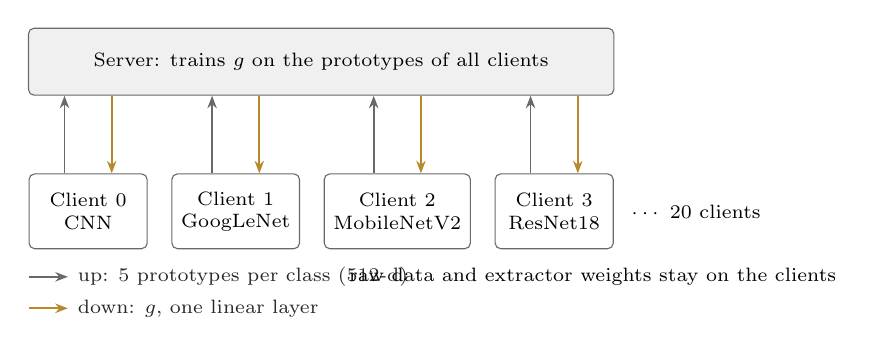
\begin{tikzpicture}[font=\scriptsize,
  cl/.style={draw=ink!70, rounded corners=2pt, align=center, minimum width=1.5cm, minimum height=0.95cm, fill=white},
  arr/.style={-{Stealth[length=1.6mm]}, draw=ink!70, line width=0.6pt}]
\node[cl] (c1) {Client 0\\CNN};
\node[cl, right=0.3cm of c1] (c2) {Client 1\\GoogLeNet};
\node[cl, right=0.3cm of c2] (c3) {Client 2\\MobileNetV2};
\node[cl, right=0.3cm of c3] (c4) {Client 3\\ResNet18};
\node[right=0.1cm of c4] (dots) {$\cdots$ 20 clients};
\node[draw=ink!70, rounded corners=2pt, fill=black!6, align=center, minimum height=0.85cm,
      fit={($(c1.west)+(0,1.9)$) ($(c4.east)+(0,1.9)$)}, inner sep=0pt] (s) {};
\node at (s.center) {Server: trains $g$ on the prototypes of all clients};
\foreach \c in {c1,c2,c3,c4} {
  \draw[arr] ([xshift=-3mm]\c.north) -- ([xshift=-3mm]\c.north |- s.south);
  \draw[arr, draw=gold] ([xshift=3mm]\c.north |- s.south) -- ([xshift=3mm]\c.north);
}
\draw[arr] ($(c1.south west)+(0,-0.35)$) -- ++(0.5,0) node[right, text=ink] {up: 5 prototypes per class (512-d)};
\draw[arr, draw=gold] ($(c1.south west)+(0,-0.75)$) -- ++(0.5,0) node[right, text=ink] {down: $g$, one linear layer};
\node[anchor=west] at ($(c3.south west)+(0.2,-0.35)$) {raw data and extractor weights stay on the clients};
\end{tikzpicture}}
\caption{Communication in Fed-GDBD. Each client uploads $k$-means prototypes of its own features and receives $g$; it never shares data or extractor weights. The 20 clients cycle through four architectures.}
\label{fig:system}
\end{figure}

\subsection{The four steps of a round}
\textit{Pre-training.} Each client first trains its model with cross-entropy. The paper starts from trained local models without saying for how long; we use 5 epochs. Each client then sends its head once, to initialise $g$.

\textit{Local training with IKD.} In every round each client trains for 5 epochs with
\begin{equation}
\begin{split}
\mathcal{L}_{\text{local}} = {}&\mathrm{CE}\big(h_i(z), y\big)\\
&+ T^2\,\mathrm{KL}\big(\sigma(\bar{u}^{t}/T)\,\big\|\,\sigma(\bar{u}^{s}/T)\big),
\end{split}
\label{eq:local}
\end{equation}
where $u^s$ are the logits of the current model, $u^t$ those of the client's best earlier model, and the bar means the true class has been removed before the softmax (we set its logit to $-10^4$). The term transfers only the ranking of the wrong classes and has zero gradient on the true class.

\textit{Multi-prototypes.} After local training, the client clusters the features of each class $c$ it holds:
\begin{equation}
\begin{split}
\{P_{c,1},\dots,P_{c,v}\} &= \text{k-means++}\big(S_c,\, v\big),\quad v=5,\\
S_c &= \{f_i(x) : (x,y)\in D_i,\ y=c\},
\end{split}
\label{eq:protos}
\end{equation}
with at most 100 iterations, and uploads at most $5C$ vectors of 512 numbers.

\textit{Global decision boundary.} The server initialises $g$ once as the sample-weighted average of the heads, $\theta_g^{(0)}=\sum_i \frac{n_i}{n}\theta_{h_i}$ (Eq.~5 of \cite{zhang2025gdbd}), and in every round trains it with cross-entropy on the union $\mathcal{P}$ of all prototypes (Eq.~12 of \cite{zhang2025gdbd}):
\begin{equation}
\min_{g} \sum_{(P,c)\in\mathcal{P}} \mathrm{CE}\big(g(P), c\big),
\label{eq:gtrain}
\end{equation}
using SGD with learning rate 0.01 and batch size 10 for 5 epochs, continuing from the previous round's $g$.

\textit{Distillation update.} Each client receives $g$, keeps it frozen and trains for 5 epochs with (Eq.~13 of \cite{zhang2025gdbd})
\begin{equation}
\begin{split}
\mathcal{L}_{\text{update}} = {}&(1-\alpha)\,\mathrm{CE}\big(h_i(z),y\big)\\
&+ \alpha T^2\,\mathrm{KL}\big(\sigma(g(z)/T)\,\big\|\,\sigma(h_i(z)/T)\big),
\end{split}
\label{eq:update}
\end{equation}
with $\alpha=0.7$ and $T=20$, so the KD term carries a weight of $\alpha T^2=280$ against $0.3$ for cross-entropy. The client is then evaluated, and if it beats its best model so far it becomes the new IKD teacher. Fig.~\ref{fig:pipeline} shows the whole round, including the two gates of Section~\ref{sec:gates}.

\begin{figure}[t]
\centering
\resizebox{\columnwidth}{!}{%
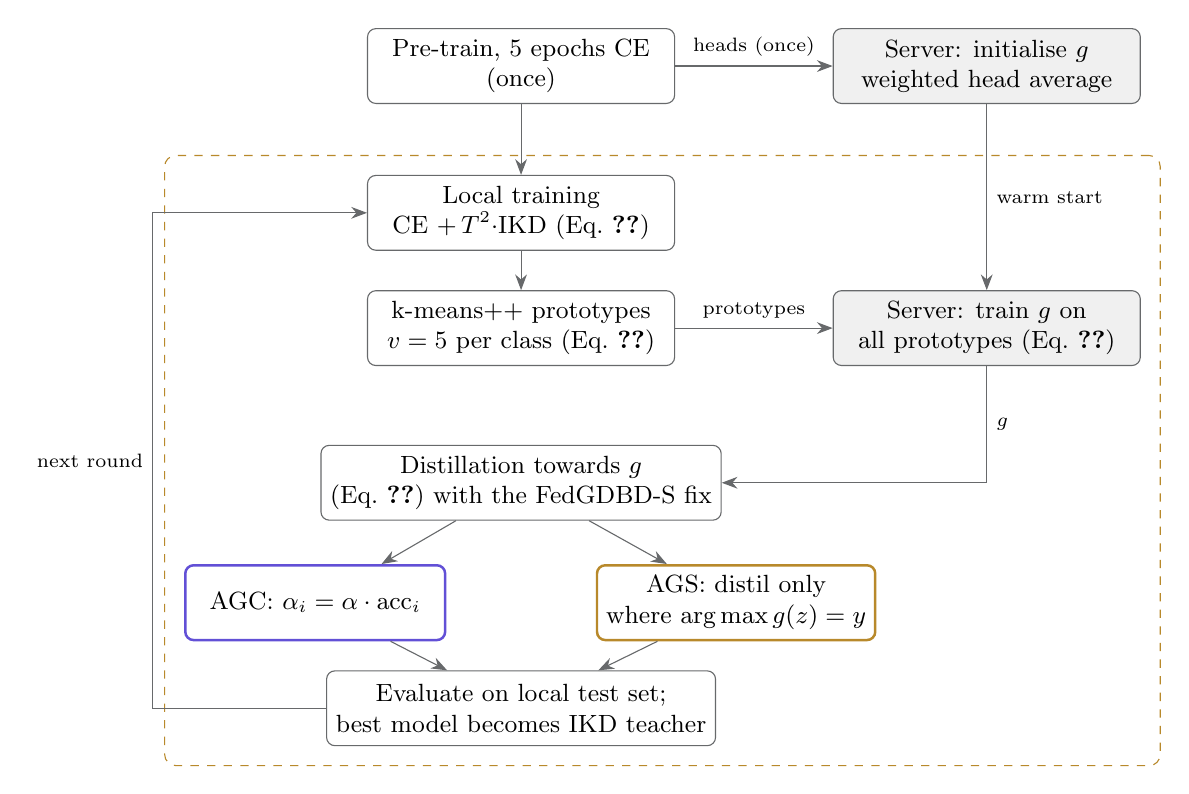
\begin{tikzpicture}[
  font=\small, node distance=0.5cm,
  box/.style={draw=ink!70, rounded corners=3pt, align=center, minimum width=3.9cm, minimum height=0.95cm, fill=white},
  srv/.style={box, fill=black!6},
  agc/.style={box, draw=violet, line width=0.9pt, minimum width=3.3cm},
  ags/.style={box, draw=gold, line width=0.9pt, minimum width=3.3cm},
  arr/.style={-{Stealth[length=2mm]}, draw=ink!70}]
\node[box] (pre) {Pre-train, 5 epochs CE\\(once)};
\node[box, below=0.9cm of pre] (loc) {Local training\\CE $+\,T^2\cdot$IKD (Eq.~\ref{eq:local})};
\node[box, below=of loc] (pro) {k-means++ prototypes\\$v=5$ per class (Eq.~\ref{eq:protos})};
\node[srv, right=2.0cm of pre] (ini) {Server: initialise $g$\\weighted head average};
\node[srv, right=2.0cm of pro] (trg) {Server: train $g$ on\\all prototypes (Eq.~\ref{eq:gtrain})};
\node[box, below=1.0cm of pro] (fix) {Distillation towards $g$\\(Eq.~\ref{eq:update}) with the FedGDBD-S fix};
\node[agc, below left=0.55cm and -1.6cm of fix] (a) {AGC: $\alpha_i=\alpha\cdot\mathrm{acc}_i$};
\node[ags, below right=0.55cm and -1.6cm of fix] (b) {AGS: distil only\\where $\arg\max g(z)=y$};
\node[box, below=1.9cm of fix] (ev) {Evaluate on local test set;\\best model becomes IKD teacher};
\draw[arr] (pre) -- (loc);
\draw[arr] (loc) -- (pro);
\draw[arr] (pre) -- node[above, font=\scriptsize]{heads (once)} (ini);
\draw[arr] (ini) -- node[right, font=\scriptsize]{warm start} (trg);
\draw[arr] (pro) -- node[above, font=\scriptsize]{prototypes} (trg);
\draw[arr] (trg) |- node[pos=0.25, right, font=\scriptsize]{$g$} (fix);
\draw[arr] (fix) -- (a); \draw[arr] (fix) -- (b);
\draw[arr] (a) -- (ev); \draw[arr] (b) -- (ev);
\draw[arr] (ev.west) -- ++(-2.2,0) |- node[pos=0.25, left, font=\scriptsize]{next round} (loc.west);
\begin{scope}[on background layer]
\node[draw=gold, dashed, rounded corners=4pt, inner sep=7pt, fit=(loc)(pro)(trg)(fix)(a)(b)(ev)] {};
\end{scope}
\end{tikzpicture}}
\caption{One round of the implemented method. Everything inside the dashed box repeats every round; shaded boxes run on the server. The two gated variants (AGC, AGS) change only the distillation step; Fed-GDBD itself uses a fixed $\alpha$.}
\label{fig:pipeline}
\end{figure}

% =====================================================================
\section{Reproduction}
\label{sec:repro}

\subsection{Implementation and assumptions}
We built on HtFLlib \cite{zhang2025htfllib}, which provides the training loop, the four models (its \texttt{HtFE-img-4} family), FedProto, LG-FedAvg and evaluation. Fed-GDBD is not in HtFLlib, so the client (\texttt{clientgdbd.py}, 299 lines) and server (\texttt{servergdbd.py}, 102 lines) are ours, written from the paper's equations. Clients and server exchange models, prototypes and $g$ through files, as HtFLlib simulates communication on one machine. Table~\ref{tab:assumptions} lists the decisions the paper left open. We chose the simplest reading consistent with the text and kept each choice fixed for all runs.

\begin{table}[t]
\centering
\caption{Assumptions where the paper gives no detail.}
\label{tab:assumptions}
\footnotesize
\begin{tabularx}{\columnwidth}{>{\raggedright\arraybackslash}p{2.6cm}>{\raggedright\arraybackslash}X}
\toprule
Detail & Our choice \\
\midrule
Length of pre-training & 5 epochs of cross-entropy \\
IKD teacher & client's past model with the best accuracy (test set in the reproduction; a 10\% validation slice in the extension) \\
$g$ during distillation & frozen; only the client learns \\
Training of $g$ & SGD, lr 0.01, batch 10, 5 epochs per round, warm start \\
Masking in IKD & true-class logit set to $-10^4$ before the softmax \\
FedProto weight $\lambda$ & 10 (HtFLlib default) \\
Classes with $\le 5$ images & their features are sent as prototypes \\
\bottomrule
\end{tabularx}
\end{table}

\subsection{Experimental setup}
Table~\ref{tab:setup} compares our setup with the paper's. The clients, models, split and hyper-parameters are the same. We reduced the datasets, rounds and repeats: the paper's full grid amounts to roughly 1,500 GPU-hours, and we had an RTX~3050 (6~GB) and an RTX~5060 (8~GB) laptop GPU, with three runs sharing one GPU at a time. The reported metric is HtFLlib's averaged test accuracy, which pools all 20 clients' test sets, at the best round, as in the paper. Accuracy per architecture is the mean over the five clients that run it.

\begin{table*}[t]
\centering
\caption{Experimental setup: the paper and ours. The difference in rounds and repeats is the main limitation of our study (Section~\ref{sec:limits}).}
\label{tab:setup}
\footnotesize
\begin{tabularx}{\textwidth}{>{\raggedright\arraybackslash}p{2.6cm}>{\raggedright\arraybackslash}X>{\raggedright\arraybackslash}X}
\toprule
 & Paper \cite{zhang2025gdbd} & Ours \\
\midrule
Datasets & CIFAR-10, CIFAR-100, Tiny-ImageNet, Flowers102 & CIFAR-10 and CIFAR-100 \cite{krizhevsky2009cifar} \\
Split & Dirichlet $\beta=0.1$ (practical) and pathological & Dirichlet $\beta=0.1$ over 20 clients, 75\% train / 25\% test per client \\
Clients and models & 20; CNN, GoogLeNet, MobileNetV2, ResNet18 & same; client $i$ runs model $i \bmod 4$ \\
Hyper-parameters & batch 10, lr 0.01, 5 local epochs, $v=5$, $\alpha=0.7$, $T=20$ & same \\
Methods & Fed-GDBD, FedProto, FedTGP, LG-FedAvg, FedGH & Fed-GDBD, FedProto, LG-FedAvg; FedGDBD-S, AGC, AGS, matched-$\alpha$ control \\
\textbf{Rounds $\times$ repeats} & \textbf{100 rounds $\times$ 3 runs} & \textbf{reproduction: 50 rounds $\times$ 1 run; extension: 20 rounds $\times$ \NSeeds{} seeds} \\
Metric & mean local test accuracy at the best round & same \\
\bottomrule
\end{tabularx}
\end{table*}

\subsection{Comparison with the paper}
Table~\ref{tab:repro} compares our best-round accuracies with Table~1 of the paper. Both baselines land close to the published values: FedProto is 0.23 pt below on CIFAR-10, and LG-FedAvg 0.28 and 0.51 pt below. The exception is FedProto on CIFAR-100, 4.13 pt above the paper. We do not know the cause; candidates are HtFLlib's default $\lambda=10$, a different draw of the random split, and best-round reporting from a single run. Since the other three baseline numbers agree, we do not think it points to a problem in the pipeline.

The faithful Fed-GDBD reaches 85.70\% and 40.70\%, 2.20 and 4.39 pt below the paper. These are its best rounds, round 1 and round 2, after which it degrades (Section~\ref{sec:collapse}). With our fix, FedGDBD-S reaches 87.10\% and 43.74\%. This is the best of the four methods on both datasets and 0.74 and 0.95 pt above LG-FedAvg, but still 0.80 and 1.35 pt below the paper's Fed-GDBD, with half the rounds and one run. We beat our own literal implementation, not the paper's reported numbers.

\begin{table}[t]
\centering
\caption{Best-round averaged test accuracy (\%) of our runs and the paper's, practical setting, 50 rounds, one run. $\Delta$ = ours $-$ paper. For FedGDBD-S the paper column repeats the paper's Fed-GDBD. $^\dagger$Best round before the collapse.}
\label{tab:repro}
\footnotesize
\setlength{\tabcolsep}{3.2pt}
\resizebox{\columnwidth}{!}{\TabReproMain}
\end{table}

Table~\ref{tab:runs} gives the details of each run. For the three stable methods, last and best differ by at most 0.49 pt. The spread across clients is large for every method (about 13 pt on CIFAR-10 and 6 to 9 pt on CIFAR-100) because some clients hold easier classes than others. FedGDBD-S takes about 10 minutes per round, against 5 to 10 for the baselines, because each round has two local training phases and a clustering step. Fig.~\ref{fig:repro_conv} shows the accuracy over the 50 rounds. Both Fed-GDBD versions start high because they begin from pre-trained models, and are within 1 pt of their best by round 2 to 5, while the baselines need 13 to 31 rounds. We do not count this as a pure advantage of the method, since the baselines start from untrained models.

\begin{table*}[t]
\centering
\caption{Details of each reproduction run. Client SD = standard deviation of the 20 clients' accuracies at the best round (pt); Min/rd. = average minutes per round with three runs sharing one GPU.}
\label{tab:runs}
\footnotesize
\TabReproRuns
\end{table*}

\begin{figure*}[t]
\centering
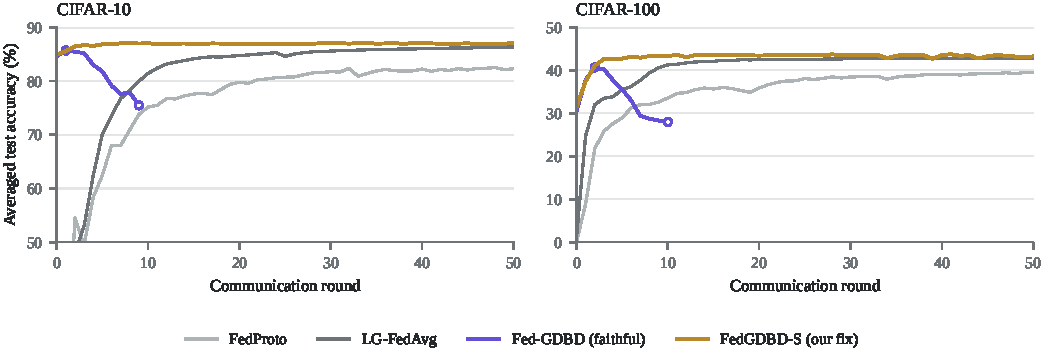
\includegraphics[width=\textwidth]{figures/repro_convergence.pdf}
\caption{Averaged test accuracy over 50 rounds. On the faithful Fed-GDBD line, the filled dot marks its best round and the open dot the round at which we stopped it.}
\label{fig:repro_conv}
\end{figure*}

\subsection{The collapse of the literal update}
\label{sec:collapse}
Breaking the accuracy down by architecture shows where the literal update fails (Table~\ref{tab:collapse}, Fig.~\ref{fig:collapse}). On CIFAR-100 the CNN clients fall from 48.0\% at round 2 to 3.9\% at round 10, and the ResNet18 clients from 35.7\% to 25.4\%, while the GoogLeNet and MobileNetV2 clients keep improving. On CIFAR-10 the ResNet18 clients suffer most, from 78.7\% to 53.3\%; CNN and GoogLeNet clients lose about 8 pt each, and MobileNetV2 clients gain 2.3 pt. So the damage is uneven across architectures and different on the two datasets. We stopped the faithful runs after 9 and 10 rounds, once the decline was clear.

\begin{table}[t]
\centering
\caption{Mean test accuracy (\%) of the five clients of each architecture: faithful Fed-GDBD at its best and last rounds, and FedGDBD-S at round 50.}
\label{tab:collapse}
\footnotesize
\setlength{\tabcolsep}{2.6pt}
\resizebox{\columnwidth}{!}{\TabCollapse}
\end{table}

\begin{figure*}[t]
\centering
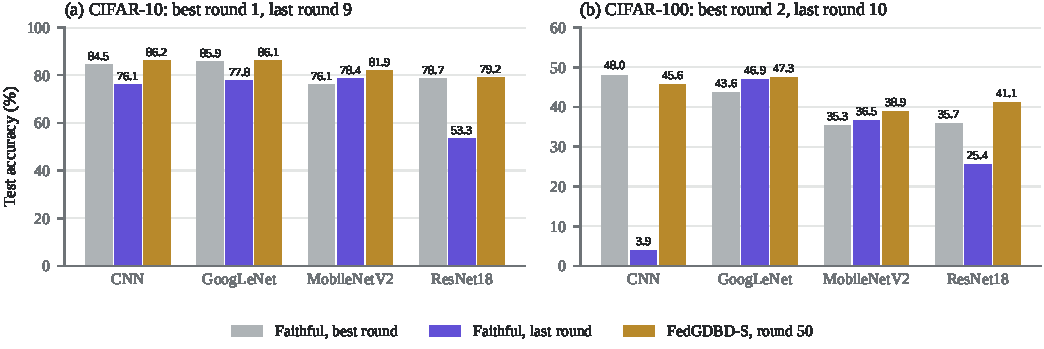
\includegraphics[width=\textwidth]{figures/repro_collapse.pdf}
\caption{Accuracy per client architecture for the faithful Fed-GDBD at its best and last rounds, and for FedGDBD-S at round 50. (a) CIFAR-10: ResNet18 clients fall from 78.7\% to 53.3\%. (b) CIFAR-100: CNN clients fall from 48.0\% to 3.9\%. FedGDBD-S ends at or above the faithful run's best for every architecture.}
\label{fig:collapse}
\end{figure*}

\textit{A bug we ruled out.} Our first IKD loss computed a softmax over all classes and then dropped the true class from the KL sum. That looks equivalent but is not: the true-class logit still enters the normalisation, so the loss pushes the correct class down at every step. On CIFAR-100 that run peaked at round 2 (41.36\%) and crashed with a NaN loss at round 8. Removing the true-class logit before the softmax fixed the crash, but the accuracy followed almost the same decline (Fig.~\ref{fig:ikdbug}). The bug added a crash; the decline comes from Eq.~\eqref{eq:update}.

\begin{figure}[t]
\centering
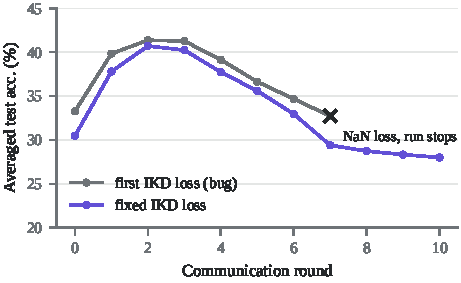
\includegraphics[width=\columnwidth]{figures/repro_ikd_bug.pdf}
\caption{CIFAR-100, faithful Fed-GDBD with our first, wrong IKD loss and with the fixed loss. Both decline after round 2; only the first one crashes.}
\label{fig:ikdbug}
\end{figure}

\subsection{The fix: FedGDBD-S}
\label{sec:fix}
Our explanation, which fits the logs but which we have not proven, is the following. $g$ is fitted to four feature spaces at once, and on some architectures its logits come out much larger than those of the client's own head. With a KD weight of 280, a confident teacher that is partly wrong for that client overwhelms cross-entropy and drags the whole model, extractor included, towards $g$'s mistakes, round after round. We made two changes and kept $\alpha$ and $T$ as in the paper:
\begin{enumerate}
\item \textit{Logit-scale matching.} Per image, $g$'s logits are rescaled to the spread of the student's:
\begin{equation}
\tilde{g}(z) = g(z)\cdot \frac{\mathrm{std}\big(h_i(\mathrm{sg}(z))\big)}{\mathrm{std}\big(g(z)\big)}.
\label{eq:scale}
\end{equation}
A positive rescaling keeps $g$'s ranking, so its top class is unchanged, but $g$ can no longer be far more confident than the student.
\item \textit{Head-only distillation.} The KD term is computed on $h_i(\mathrm{sg}(z))$, so it updates only the head. Cross-entropy still trains the whole model.
\end{enumerate}
The resulting loss is
\begin{equation}
\begin{split}
\mathcal{L}_{\text{S}} = {}&(1-\alpha)\,\mathrm{CE}\big(h_i(z),y\big)\\
&+ \alpha T^2\,\mathrm{KL}\big(\sigma(\tilde{g}(z)/T)\,\big\|\,\sigma(h_i(\mathrm{sg}(z))/T)\big).
\end{split}
\label{eq:fgs}
\end{equation}
We made this fix during the reproduction; it is not our extension, but it is the base the extension builds on and the control it is compared with. FedGDBD-S shows no downward trend over 50 rounds: from round 3 on, its accuracy never drops more than 0.53 pt below its best on CIFAR-10 and 1.1 pt on CIFAR-100, and its last-round accuracies are 87.06\% and 43.25\%.

\subsection{Per-architecture accuracy of all methods}
Fig.~\ref{fig:archmethods} and Table~\ref{tab:archmethods} compare all four methods per architecture at their best rounds. FedProto is the strongest method on CNN clients (87.1\% and 51.4\%) and the weakest on MobileNetV2 (68.6\% and 29.7\%), which suggests that pulling features towards one global mean per class suits some extractors far better than others. FedGDBD-S is the best on MobileNetV2 on both datasets (81.6\% and 38.8\%). MobileNetV2 is the hardest architecture for every method.

\begin{figure*}[t]
\centering
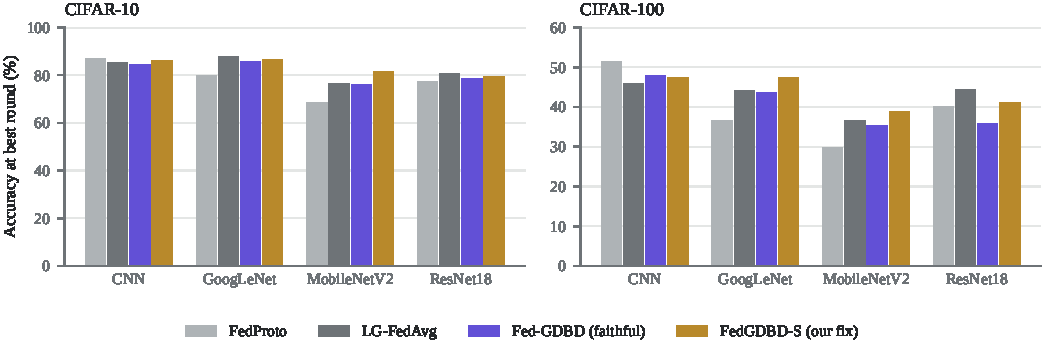
\includegraphics[width=\textwidth]{figures/repro_arch_methods.pdf}
\caption{Accuracy per client architecture for the four methods at their best rounds.}
\label{fig:archmethods}
\end{figure*}

\begin{table}[t]
\centering
\caption{Mean test accuracy (\%) per architecture for each method at its best round.}
\label{tab:archmethods}
\footnotesize
\setlength{\tabcolsep}{2.4pt}
\resizebox{\columnwidth}{!}{\TabArchMethods}
\end{table}

% =====================================================================
\section{Agreement-Gated Distillation}
\label{sec:gates}

Our extension asks one question for each client: on this client's own features, does $g$ give the right label? $g(z)$ is already computed for the distillation and the client knows its labels, so the answer costs no communication.

\subsection{Per client (AGC)}
Before the update of each round, the client measures $g$'s accuracy on its own training data in one pass without gradients and scales $\alpha$ by it:
\begin{equation}
\begin{split}
\mathrm{acc}_i &= \frac{1}{|D_i|}\sum_{(x,y)\in D_i} \mathbf{1}\big[\arg\max g(f_i(x)) = y\big],\\
\alpha_i &= \alpha\cdot\mathrm{acc}_i.
\end{split}
\label{eq:agc}
\end{equation}
The update then uses Eq.~\eqref{eq:fgs} with $\alpha_i$ in place of $\alpha$. A client whose features $g$ reads well keeps a weight close to the paper's 0.7; a client that $g$ misreads leans more on its own labels. The extra cost is one forward pass per round.

\subsection{Per sample (AGS)}
AGS makes the same check for every image:
\begin{equation}
\begin{aligned}
w &= \mathbf{1}\big[\arg\max \tilde{g}(z) = y\big],\\
\mathcal{L}_{\text{AGS}} &= \operatorname{mean}\Big[(1-\alpha w)\,\mathrm{CE}\big(h_i(z),y\big)\\
&\qquad + \alpha w\, T^2\,\mathrm{KL}\big(\sigma(\tilde{g}/T)\,\|\,\sigma(h_i(\mathrm{sg}(z))/T)\big)\Big].
\end{aligned}
\label{eq:ags}
\end{equation}
Where $g$ is right ($w=1$) the loss is that of FedGDBD-S; where it is wrong ($w=0$) the image gets plain cross-entropy. The gates differ in what they do with the images $g$ gets wrong: AGC still distils them at a lower weight, while AGS ignores $g$ on them. AGS costs nothing extra. Fig.~\ref{fig:gate} shows the test both gates use, and Algorithm~\ref{alg:update} gives the client update in all four versions; it follows the \texttt{update()} function of our code line for line.

\begin{figure}[t]
\centering
\resizebox{\columnwidth}{!}{%
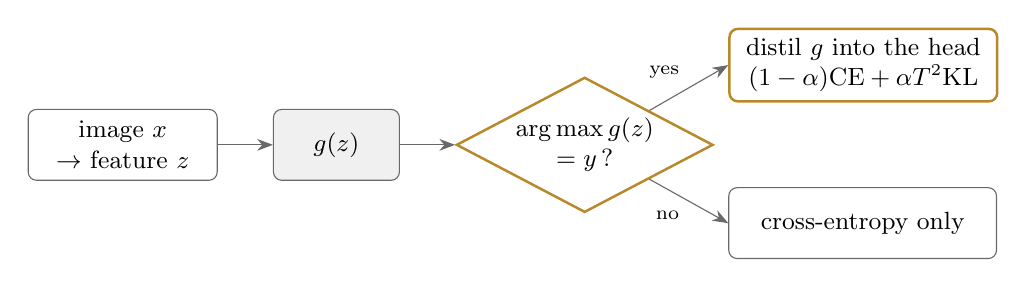
\begin{tikzpicture}[font=\small,
  box/.style={draw=ink!70, rounded corners=3pt, align=center, minimum height=0.9cm, fill=white},
  arr/.style={-{Stealth[length=2mm]}, draw=ink!70}]
\node[box, minimum width=2.4cm] (x) {image $x$\\$\to$ feature $z$};
\node[box, fill=black!6, minimum width=1.6cm, right=0.7cm of x] (g) {$g(z)$};
\node[draw=gold, line width=0.9pt, diamond, aspect=1.9, inner sep=1pt, align=center, right=0.7cm of g] (d) {$\arg\max g(z)$\\$= y$\,?};
\node[box, draw=gold, line width=0.9pt, minimum width=3.4cm, above right=0.1cm and 1.0cm of d] (yes) {distil $g$ into the head\\$(1-\alpha)\mathrm{CE} + \alpha T^2 \mathrm{KL}$};
\node[box, minimum width=3.4cm, below right=0.1cm and 1.0cm of d] (no) {cross-entropy only};
\draw[arr] (x) -- (g); \draw[arr] (g) -- (d);
\draw[arr] (d.north east) -- node[above left, font=\scriptsize]{yes} (yes.west);
\draw[arr] (d.south east) -- node[below left, font=\scriptsize]{no} (no.west);
\end{tikzpicture}}
\caption{The agreement test. AGS applies it to every image. AGC averages its answer over a client's training images and scales $\alpha$ by the result.}
\label{fig:gate}
\end{figure}

\begin{algorithm}[t]
\caption{Client distillation step in all four versions}
\label{alg:update}
\footnotesize
\begin{algorithmic}[1]
\State $\alpha \gets 0.7$ \Comment{all}
\If{gate = client} $\alpha \gets \alpha \cdot \mathrm{acc}_i(g)$ \Comment{AGC}
\EndIf
\For{5 epochs, each batch $(x,y)$ of $D_i$}
  \State $z \gets f_i(x)$; $o \gets h_i(z)$; $q \gets g(z)$ without gradient
  \If{stable} \Comment{S, AGC, AGS}
    \State $k \gets h_i(\mathrm{sg}(z))$; $q \gets q\cdot\mathrm{std}(k)/\mathrm{std}(q)$
  \Else\ $k \gets o$ \Comment{faithful}
  \EndIf
  \If{gate = sample} \Comment{AGS}
    \State $w \gets [\arg\max q = y]$
    \State $\mathcal{L} \gets \mathrm{mean}\big((1-\alpha w)\mathrm{CE}(o,y) + \alpha w T^2\mathrm{KL}(q\|k)\big)$
  \Else\ $\mathcal{L} \gets (1-\alpha)\mathrm{CE}(o,y) + \alpha T^2\mathrm{KL}(q\|k)$
  \EndIf
  \State SGD step on $\mathcal{L}$, gradient norm clipped at 10
\EndFor
\end{algorithmic}
\end{algorithm}

\subsection{Communication and cost}
None of our changes sends anything new. On CIFAR-100 a client uploads at most 500 prototypes of 512 floats per round (about 1~MB) and receives $g$ with $512\times100+100$ parameters (about 0.2~MB); for comparison, ResNet18 alone has about 11 million parameters. Table~\ref{tab:versions} summarises the versions.

\begin{table}[t]
\centering
\caption{The versions of the client update compared in this paper.}
\label{tab:versions}
\footnotesize
\begin{tabularx}{\columnwidth}{>{\raggedright\arraybackslash}p{1.9cm}>{\raggedright\arraybackslash}X}
\toprule
Version & Distillation step \\
\midrule
Fed-GDBD (faithful) & Eq.~\eqref{eq:update}: fixed $\alpha=0.7$, KD trains the whole model \\
FedGDBD-S & Eq.~\eqref{eq:fgs}: logit-scale matching, head-only KD; the control \\
Matched $\alpha$ & Eq.~\eqref{eq:fgs} with one lower $\alpha$ for all clients (Section~\ref{sec:protocol}) \\
FedGDBD-AGC & Eq.~\eqref{eq:fgs} with $\alpha_i=0.7\cdot\mathrm{acc}_i$ \\
FedGDBD-AGS & Eq.~\eqref{eq:ags}: distil only where $g$'s top class is the label \\
\bottomrule
\end{tabularx}
\end{table}

% =====================================================================
\section{Extension Experiments}
\label{sec:ext}

\subsection{Protocol}
\label{sec:protocol}
The extension runs use a different protocol from the reproduction, and their numbers should not be compared with Section~\ref{sec:repro}.
\begin{itemize}
\item \textit{Teacher.} The IKD teacher is chosen on a fixed 10\% validation slice of each client's training data, so no test data influences training. Clients train on the other 90\%.
\item \textit{Seeds and rounds.} Each method runs for 20 rounds with seeds \SeedList{}. The seed controls model initialisation, client order and k-means seeding; the data split is fixed. We used 20 rounds because FedGDBD-S had converged by then in the 50-round runs (its best accuracy in the first 20 rounds was within 0.1 pt of its best over 50) and because it made several seeds affordable. One set of three runs took 5 to 6.5 hours on one laptop GPU.
\item \textit{Matched-$\alpha$ control.} AGC lowers the average distillation weight, so any gain could come simply from a lower $\alpha$. To separate the two, we run FedGDBD-S with one fixed $\alpha$ for all clients, equal to the mean $\alpha_i$ that AGC used over all clients and rounds in seeds 0 and 1: 0.58 on CIFAR-10 and 0.49 on CIFAR-100.
\item \textit{Fixed in advance.} After seeds 0 and 1, and before running seeds 2 and 3 or the matched-$\alpha$ control, we committed a protocol to the public repository. It fixes the seeds, the matched $\alpha$ values, the metric, three hypotheses and the tests. H1: AGC beats the control on CIFAR-100. H2: AGC beats the matched-$\alpha$ control on CIFAR-100. H3: AGS beats the control on CIFAR-10. Each is tested with a one-sided paired $t$-test over seeds; other comparisons are reported with two-sided tests. The hypotheses came from seeds 0 and 1, so seeds 2 and 3 are the out-of-sample check. Our earlier success criterion, a gain of at least 0.5 pt on both datasets, was also kept.
\end{itemize}

\subsection{Main results}
Table~\ref{tab:extmain} gives the mean and standard deviation over \NSeeds{} seeds at the best round and at round 20, and Fig.~\ref{fig:extconv} the accuracy over the rounds. On CIFAR-10, AGC has higher mean best-round accuracy than the control (\GTenAgcCtlBest{} pt), and so does AGS (\GTenAgsCtlBest{} pt). On CIFAR-100, AGC has higher mean accuracy than the control (\GHunAgcCtlBest{} pt), while AGS is lower (\GHunAgsCtlBest{} pt). Against the matched-$\alpha$ control, both gates have higher mean accuracy on CIFAR-10 (AGC \GTenAgcAmBest{}, AGS \GTenAgsAmBest{} pt), and on CIFAR-100 only AGC does (\GHunAgcAmBest{} pt). At round 20 the picture is the same, except that AGC and the matched-$\alpha$ control are level on CIFAR-100 (\GHunAgcAmLast{} pt).

These gaps are small. Every one of them is smaller than the spread across seeds, and Fig.~\ref{fig:gaps} shows that most comparisons go one way in some seeds and the other way in others.

\begin{table}[t]
\centering
\caption{Extension runs: averaged test accuracy (\%), mean $\pm$ SD over seeds \SeedList{}, 20 rounds, validation-slice teacher. Bold: highest mean in each column.}
\label{tab:extmain}
\footnotesize
\setlength{\tabcolsep}{2.2pt}
\resizebox{\columnwidth}{!}{\TabExtMain}
\end{table}

\begin{figure*}[t]
\centering
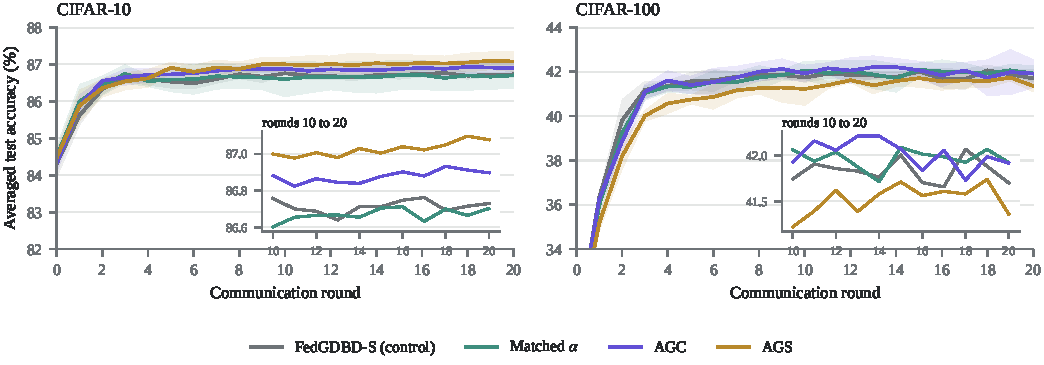
\includegraphics[width=\textwidth]{figures/ext_convergence.pdf}
\caption{Extension runs: averaged test accuracy over 20 rounds, mean over seeds \SeedList{} with a band of $\pm$1 SD. The insets enlarge rounds 10 to 20.}
\label{fig:extconv}
\end{figure*}

\begin{figure*}[t]
\centering
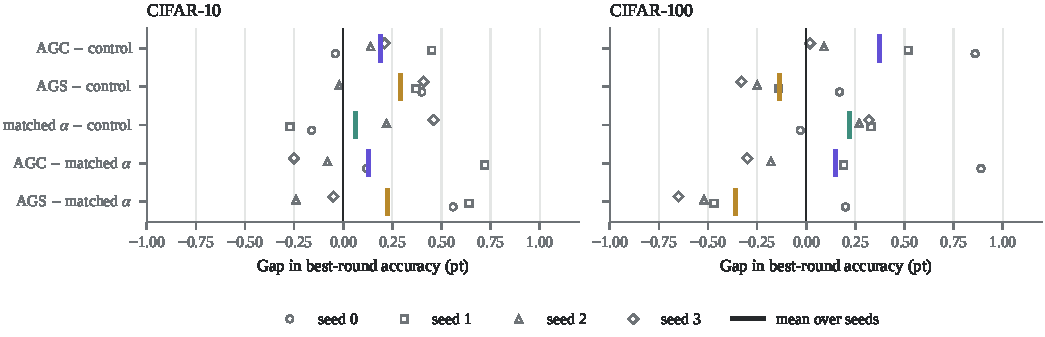
\includegraphics[width=\textwidth]{figures/ext_gaps.pdf}
\caption{Paired gaps in best-round accuracy for every seed (markers) and their mean (bar). A gap above zero means the first method was better in that seed.}
\label{fig:gaps}
\end{figure*}

\subsection{Tests fixed in advance}
Table~\ref{tab:tests} gives the paired tests. H3, AGS against the control on CIFAR-10, has a mean gap of \GTenAgsCtlBest{} pt, AGS wins in \GTenAgsCtlBestWins{} seeds, and the one-sided $p$ is \GTenAgsCtlBestPone{}. With a Holm correction for three hypotheses it becomes \HolmThree{}, and the gaps in the new seeds were mixed (\GTenAgsCtlBestNew{}). H1, AGC against the control on CIFAR-100, has a mean gap of \GHunAgcCtlBest{} pt and AGC wins in \GHunAgcCtlBestWins{} seeds, but $p=\GHunAgcCtlBestPone{}$. Its per-seed gains were \GHunAgcCtlBestSeeds{}, so the mean is carried mostly by seeds 0 and 1. H2, AGC against the matched-$\alpha$ control on CIFAR-100, is not supported ($p=\GHunAgcAmBestPone{}$); in the new seeds the matched control was ahead (\GHunAgcAmBestNew{}). Neither gate met the 0.5 pt criterion on both datasets.

\begin{table*}[t]
\centering
\caption{Paired comparisons of best-round accuracy over seeds \SeedList{}. Mean gap and 95\% confidence interval in pt; $p$ from a paired $t$-test, one-sided (1s) for the hypotheses fixed in advance and two-sided (2s) otherwise; wins = seeds in which the first method is better; last column = mean gap over the new seeds only (2 and later).}
\label{tab:tests}
\footnotesize
\TabTests
\end{table*}

\textit{The lower distillation weight on its own.} The protocol did not include a test of the matched-$\alpha$ control against the plain control, so we report it only descriptively: its mean gap is \GTenAmCtlBest{} pt on CIFAR-10 and \GHunAmCtlBest{} pt on CIFAR-100. On CIFAR-100, then, simply lowering $\alpha$ gives a gain of similar size to AGC's, which is why H2 fails.

\subsection{Per architecture}
Fig.~\ref{fig:archgain} and Table~\ref{tab:archgain} break the gains down by architecture. On CIFAR-10 the MobileNetV2 clients gain the most from AGS (\GainTenAgsMob{} pt) and AGC (\GainTenAgcMob{} pt), while the matched $\alpha$ gives them nothing (\GainTenAmMob{} pt). On CIFAR-100, AGC and the matched $\alpha$ both help MobileNetV2 (\GainHunAgcMob{} and \GainHunAmMob{} pt) and ResNet18 (\GainHunAgcRes{} and \GainHunAmRes{} pt); the matched $\alpha$ costs the CNN clients more than AGC does (\GainHunAmCnn{} against \GainHunAgcCnn{} pt), which fits the design, since AGC keeps a higher weight for clients that $g$ reads well. AGS costs the CIFAR-100 CNN clients \GainHunAgsCnn{} pt, which explains why it does not help there overall.

\begin{figure*}[t]
\centering
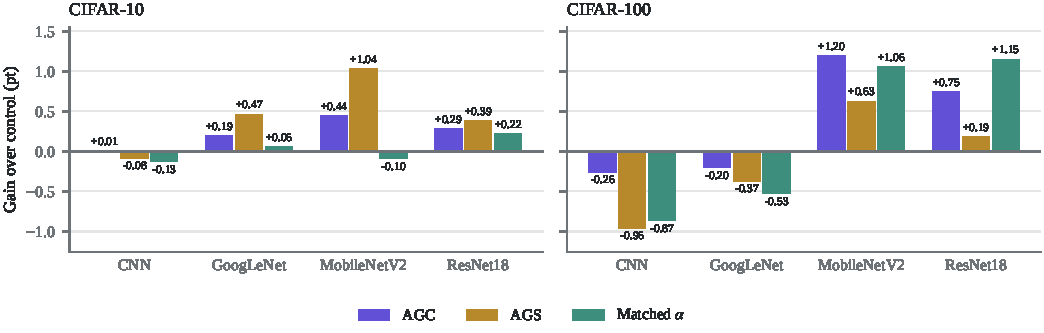
\includegraphics[width=\textwidth]{figures/ext_arch_gains.pdf}
\caption{Gain over the control per client architecture at the best round, mean over seeds \SeedList{}.}
\label{fig:archgain}
\end{figure*}

\begin{table}[t]
\centering
\caption{Gain over the control per architecture (pt), mean over seeds \SeedList{}, best round.}
\label{tab:archgain}
\footnotesize
\setlength{\tabcolsep}{2.6pt}
\resizebox{\columnwidth}{!}{\TabArchGain}
\end{table}

\subsection{What the gates measured}
The gate statistics describe how well $g$ fits each architecture (Table~\ref{tab:gate}, Figs.~\ref{fig:gacc} and~\ref{fig:kept}). Averaged over the rounds, $g$ classifies \GaccTenCnn{} of the CNN clients' CIFAR-10 training images correctly but only \GaccTenMob{} of the MobileNetV2 clients'. On CIFAR-100 the figures are \GaccHunCnn{} to \GaccHunRes{} for CNN, GoogLeNet and ResNet18 against \GaccHunMob{} for MobileNetV2. At round 0 the gap is extreme: $g$ is right on \GaccZeroTenMob{} of MobileNetV2 images on CIFAR-10 and \GaccZeroHunMob{} on CIFAR-100. The gate was never told about architectures, yet in every seed it singles out MobileNetV2 as the architecture $g$ serves worst. $g$'s accuracy on MobileNetV2 features rises over the run as $g$ and the clients adapt, so the gate lowers MobileNetV2's distillation weight most in the early rounds.

AGS shows the same pattern from another angle. On CIFAR-10, MobileNetV2 clients distil only \KeptTenMob{} of their images on average against \KeptTenCnn{} for CNN clients. On CIFAR-100, MobileNetV2 climbs from almost none at round 0 to almost all. These fractions are counted during training, with the model in training mode, so they differ from AGC's evaluation-mode accuracy, but both point to MobileNetV2.

\begin{table}[t]
\centering
\caption{Gate statistics per architecture, mean over seeds \SeedList{}. AGC rows: share of training images $g$ classifies correctly. AGS rows: share of images distilled.}
\label{tab:gate}
\scriptsize
\setlength{\tabcolsep}{1.8pt}
\resizebox{\columnwidth}{!}{\TabGate}
\end{table}

\begin{figure}[t]
\centering
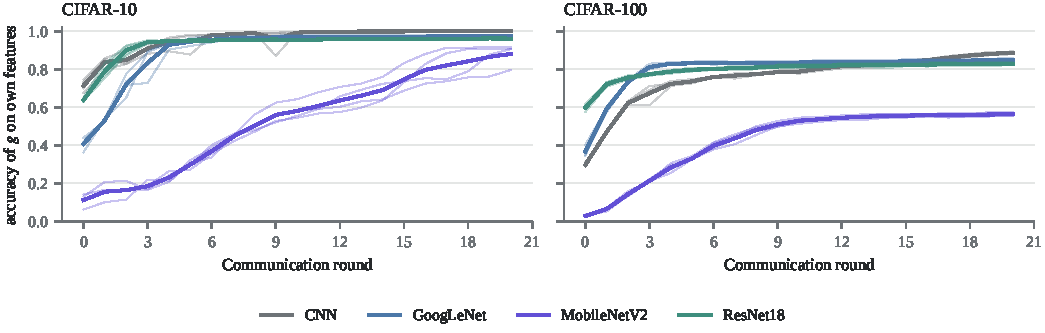
\includegraphics[width=\columnwidth]{figures/gate_gacc.pdf}
\caption{AGC: accuracy of $g$ on each architecture's own training features over the rounds. Thick lines: mean over seeds; thin lines: single seeds.}
\label{fig:gacc}
\end{figure}

\begin{figure}[t]
\centering
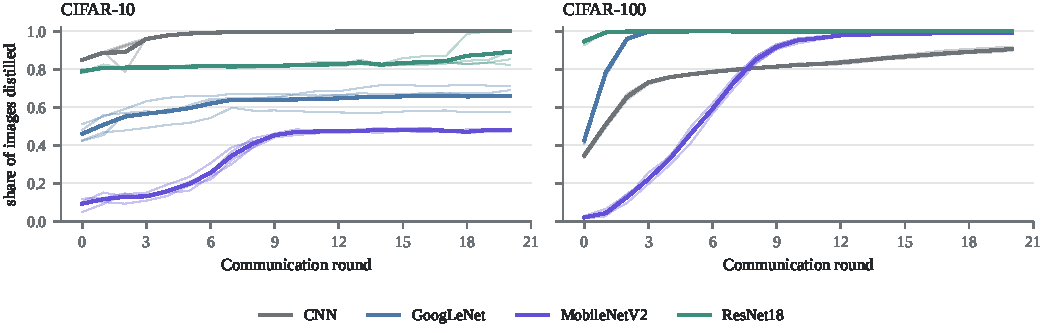
\includegraphics[width=\columnwidth]{figures/gate_kept.pdf}
\caption{AGS: share of each architecture's images distilled in each round. Thick lines: mean over seeds; thin lines: single seeds.}
\label{fig:kept}
\end{figure}

% =====================================================================
\section{Discussion}
\label{sec:discussion}

\textit{Why the literal update collapses.} The collapse hits different architectures on the two datasets and builds up over several rounds. Both facts fit a scale mismatch between $g$'s logits and some clients' heads, amplified by the KD weight $\alpha T^2=280$, so that distillation overrides cross-entropy and reshapes the extractor. The fix removes exactly these two channels, the scale and the gradient into the extractor, which supports the explanation, but we did not log logit norms to confirm it directly. The authors' code may contain a detail that avoids the problem, such as a normalisation or a smaller learning rate.

\textit{What the extension shows.} The clearest result is a measurement, not an accuracy gain: one linear boundary shared by four architectures fits them very unequally, and the difference is large. This matches the baselines, where MobileNetV2 is the hardest architecture for every method and FedProto, which also imposes one global target per class, is weakest exactly there. The accuracy results are smaller and less certain. AGS on CIFAR-10 is the only comparison below $p=0.05$, and it does not survive a correction for three hypotheses. On CIFAR-100 the matched-$\alpha$ control shows that much of AGC's gain can be had by lowering $\alpha$ for everyone, which suggests that the paper's $\alpha=0.7$ is on the high side for mixed architectures. The per-architecture results add one point in AGC's favour: it gets a similar gain on the clients $g$ serves badly while costing the well-served CNN clients less.

\textit{Why each gate suits a different dataset.} This is our interpretation and not proven. On CIFAR-100, $g$ is wrong often, but its softened predictions still say which of the 100 classes look alike, so turning distillation down smoothly (AGC) keeps that information while reducing the harm; discarding images (AGS) throws it away, and in its first rounds AGS discards almost all MobileNetV2 images. On CIFAR-10, $g$ is right on most images and there are only 10 classes, so dropping the images $g$ gets wrong cleans up the signal without losing much.

% =====================================================================
\section{Limitations}
\label{sec:limits}

\textit{Rounds and repeats.} The paper trains for 100 rounds and averages three runs. Our reproduction used 50 rounds and one run, and our extension 20 rounds per seed. For the reproduction, the comparison with the paper's numbers is therefore not like for like, and part of the remaining gap to the paper (0.80 and 1.35 pt) may come from it. For the extension, longer runs would make the comparison more rigorous, but we do not expect them to favour the gates: FedGDBD-S had converged by round 20 in our 50-round runs, and as $g$ improves on MobileNetV2 over the rounds both gates move closer to the control, AGC towards a uniform weight and AGS towards distilling every image. Whether the gaps grow or shrink with 100 rounds is an open question we have not tested.

\textit{Seeds.} \NSeeds{} seeds cannot pin down effects of a few tenths of a point; the confidence intervals in Table~\ref{tab:tests} all include zero. Seed 4 was running when this draft was written and will be added to every table and figure; the scripts regenerate them from the logs.

\textit{Scope.} We used two of the paper's four datasets, only the practical split, and two of its four baselines. We did not run a sweep over $\alpha$ and $T$; the matched-$\alpha$ control tests only one value per dataset.

\textit{Best-round reporting and the reproduction teacher.} As in the paper, the headline numbers are best-round accuracies, which are slightly optimistic; we report last-round results next to them. In the reproduction runs the IKD teacher was picked by test accuracy, as the paper implies, which is a mild use of test data shared by Fed-GDBD and FedGDBD-S; the extension runs avoid it. GPU kernels are not deterministic, so a rerun gives close but not identical numbers.

% =====================================================================
\section{Conclusion and Future Work}

We re-implemented Fed-GDBD from its paper and reproduced its main experiment on CIFAR-10 and CIFAR-100 with half the rounds and one run. The baselines matched the published numbers closely. The literal client update turned out to be unstable for particular architectures, and two changes to the distillation step fixed it without touching the paper's hyper-parameters; the fixed version was the best method in our runs and about one point below the paper's reported results.

Our extension gates the distillation of the global boundary by whether it agrees with each client's labels. Over \NSeeds{} seeds, AGC had higher mean accuracy than the control on both datasets and AGS on CIFAR-10, but the gaps were smaller than the spread across seeds, only AGS on CIFAR-10 reached $p<0.05$, and on CIFAR-100 a lower distillation weight for every client did about as well as AGC. The lasting result is the measurement behind the gates: a single global boundary fits some client architectures far worse than others, and a client can detect this from its own data at no communication cost.

Future work: (i) more seeds and the paper's 100 rounds, to measure gaps of a few tenths of a point properly; (ii) a sweep over $\alpha$ and $T$, since our control suggests $\alpha=0.7$ is high for mixed architectures; (iii) a soft gate that weights each image by $g$'s probability for the true label, and a hybrid of AGC and AGS; (iv) the paper's other datasets, the pathological split and the FedTGP and FedGH baselines; and (v) logging the logit scales of $g$ and of each head to test our explanation of the collapse.

\section*{Acknowledgment}
We thank Dr. Nagamma Patil for her guidance throughout this project, and the authors of HtFLlib and PFLlib for making their code available.

\begin{thebibliography}{99}
\bibitem{zhang2025gdbd}
K.~Zhang, J.~Wang, W.~Wang, T.~Zeng, P.~Li, X.~Wang, and T.~Zhang, ``Federated learning with heterogeneous data and models based on global decision boundary distillation,'' \emph{Journal of King Saud University -- Computer and Information Sciences}, vol.~37, art.~75, 2025, doi:10.1007/s44443-025-00097-0.

\bibitem{mcmahan2017fedavg}
B.~McMahan, E.~Moore, D.~Ramage, S.~Hampson, and B.~Ag\"{u}era y Arcas, ``Communication-efficient learning of deep networks from decentralized data,'' in \emph{Proc. Int. Conf. Artificial Intelligence and Statistics (AISTATS)}, 2017, pp.~1273--1282.

\bibitem{hsu2019noniid}
T.-M.~H.~Hsu, H.~Qi, and M.~Brown, ``Measuring the effects of non-identical data distribution for federated visual classification,'' arXiv:1909.06335, 2019.

\bibitem{liang2020lgfedavg}
P.~P.~Liang, T.~Liu, L.~Ziyin, N.~B.~Allen, R.~P.~Auerbach, D.~Brent, R.~Salakhutdinov, and L.-P.~Morency, ``Think locally, act globally: Federated learning with local and global representations,'' arXiv:2001.01523, 2020.

\bibitem{tan2022fedproto}
Y.~Tan, G.~Long, L.~Liu, T.~Zhou, Q.~Lu, J.~Jiang, and C.~Zhang, ``FedProto: Federated prototype learning across heterogeneous clients,'' in \emph{Proc. AAAI Conf. Artificial Intelligence}, 2022.

\bibitem{zhang2024fedtgp}
J.~Zhang, Y.~Liu, Y.~Hua, and J.~Cao, ``FedTGP: Trainable global prototypes with adaptive-margin-enhanced contrastive learning for data and model heterogeneity in federated learning,'' in \emph{Proc. AAAI Conf. Artificial Intelligence}, vol.~38, 2024.

\bibitem{yi2023fedgh}
L.~Yi, G.~Wang, X.~Liu, Z.~Shi, and H.~Yu, ``FedGH: Heterogeneous federated learning with generalized global header,'' in \emph{Proc. ACM Int. Conf. Multimedia (MM)}, 2023.

\bibitem{zhang2025htfllib}
J.~Zhang \emph{et al.}, ``HtFLlib: A comprehensive heterogeneous federated learning library and benchmark,'' in \emph{Proc. ACM SIGKDD Conf. Knowledge Discovery and Data Mining}, 2025.

\bibitem{zhang2025pfllib}
J.~Zhang \emph{et al.}, ``PFLlib: A beginner-friendly and comprehensive personalized federated learning library and benchmark,'' \emph{Journal of Machine Learning Research}, vol.~26, 2025.

\bibitem{hinton2015kd}
G.~Hinton, O.~Vinyals, and J.~Dean, ``Distilling the knowledge in a neural network,'' arXiv:1503.02531, 2015.

\bibitem{zhao2022dkd}
B.~Zhao, Q.~Cui, R.~Song, Y.~Qiu, and J.~Liang, ``Decoupled knowledge distillation,'' in \emph{Proc. IEEE/CVF Conf. Computer Vision and Pattern Recognition (CVPR)}, 2022.

\bibitem{arthur2007kmeanspp}
D.~Arthur and S.~Vassilvitskii, ``k-means++: The advantages of careful seeding,'' in \emph{Proc. ACM-SIAM Symp. Discrete Algorithms (SODA)}, 2007, pp.~1027--1035.

\bibitem{krizhevsky2009cifar}
A.~Krizhevsky, ``Learning multiple layers of features from tiny images,'' Technical report, University of Toronto, 2009.

\bibitem{szegedy2015googlenet}
C.~Szegedy \emph{et al.}, ``Going deeper with convolutions,'' in \emph{Proc. IEEE Conf. Computer Vision and Pattern Recognition (CVPR)}, 2015.

\bibitem{sandler2018mobilenetv2}
M.~Sandler, A.~Howard, M.~Zhu, A.~Zhmoginov, and L.-C.~Chen, ``MobileNetV2: Inverted residuals and linear bottlenecks,'' in \emph{Proc. IEEE/CVF Conf. Computer Vision and Pattern Recognition (CVPR)}, 2018.

\bibitem{he2016resnet}
K.~He, X.~Zhang, S.~Ren, and J.~Sun, ``Deep residual learning for image recognition,'' in \emph{Proc. IEEE Conf. Computer Vision and Pattern Recognition (CVPR)}, 2016.


\end{thebibliography}

% =====================================================================
\appendices

\section{Reproducing the Results}
All runs are started by Windows batch scripts in the repository, and \texttt{REPRODUCTION.md} gives the steps. \texttt{setup.bat} installs the environment. \texttt{run\_cifar10.bat} and \texttt{run\_cifar100.bat} start the reproduction runs; \texttt{run\_novelty\_cifar10\_seed$s$.bat} and \texttt{run\_novelty\_cifar100\_seed$s$.bat} start the control, AGC and AGS for seed $s$; \texttt{run\_amatch.bat} starts the matched-$\alpha$ control. The protocol of the extension runs is in \texttt{PROTOCOL.md}. Without any training, \texttt{python analysis/paper\_figures.py} regenerates every figure and results table in this paper from the logs, and \texttt{python analysis/multiseed\_summary.py} prints the paired tests.

\section{Additional Tables}

\begin{table*}[t]
\centering
\caption{Extension runs: best-round averaged test accuracy (\%) for every seed.}
\label{tab:extseeds}
\footnotesize
\TabExtSeeds
\end{table*}

\begin{table*}[t]
\centering
\caption{Extension runs: mean test accuracy (\%) per client architecture at each run's best round.}
\label{tab:extarch}
\scriptsize
\TabExtArch
\end{table*}

\begin{table*}[t]
\centering
\caption{Reproduction runs: test accuracy (\%) of each client at the best round. Left: CIFAR-10. Right: CIFAR-100.}
\label{tab:clients}
\scriptsize
\setlength{\tabcolsep}{2.6pt}
\begin{minipage}[t]{0.49\textwidth}\centering\resizebox{\linewidth}{!}{\TabClientsTen}\end{minipage}\hfill
\begin{minipage}[t]{0.49\textwidth}\centering\resizebox{\linewidth}{!}{\TabClientsHundred}\end{minipage}
\end{table*}

Table~\ref{tab:extseeds} lists every seed's best-round accuracy, Table~\ref{tab:extarch} the per-architecture accuracy of every extension run, and Table~\ref{tab:clients} each client's accuracy in the reproduction runs, which shows how much the clients differ under the skewed split.

\end{document}
